\chapter{DEVELOPMENT OF THE iOS APP}
\label{chap:development of the app}

The development of the iOS app is divided into two areas which are mentioned below.

\begin{itemize}
    \item Front-end
        \begin{itemize}
            \item App designing
            \item Mobile App screens and their significance \\
        \end{itemize}

    \item Back-end
        \begin{itemize}
            \item Process of getting data from NASA's server
            \item Web services required for \gls{json} parsing between database and the front-end \\
        \end{itemize}
        
    \item Using the App
        \begin{itemize}
            \item Data visualization
        \end{itemize}
    
     \item APIs, Softwares, Design pattern and Languages Usage
        \begin{itemize}
            \item Major APIs used
            \item Softwares used
            \item Design pattern used
            \item Software Languages used \\
        \end{itemize}    
\end{itemize}

\section{Front-end of the app}

Any part of the software or \gls{ui} that a user sees on the screen and interacts with it appropriately. It requires a lot of prior knowledge to design and program the front-end with focus on user friendliness of the app.

\subsection{App Designing}

\textbf{Xcode 9.2} has been used for the development of the app. It is an \gls{ide}, which implies it pulls every one of the instruments expected to create an application (especially a content tool, a compiler, and a manufacture framework) into one programming bundle instead of abandoning them as an arrangement of individual devices associated by contents. Xcode is Apple's authentic \gls{ide} for \gls{mac} and \gls{iOS} engineers. It was initially known as Project Builder in the NeXT days and renamed to Xcode some place around Mac OS X 10.3 or 10.4. By adaptation 4, Apple had collapsed in the sidekick Interface Builder program so there was just a single application package; the plan of the program hasn't changed a ton from that point forward, albeit clearly the instruments are refreshed routinely. \\
Apple provides Built-In Interface Builder in the \gls{ide} for designing.
According to Apple's website, The Interface Builder editor within Xcode makes it simple to design a full user interface without writing any code. Simply drag and drop windows, buttons, text fields, and other objects onto the design canvas to create a functioning user interface. \cite{Xcode} \\
Because Cocoa and Cocoa Touch are built using the Model-View-Controller pattern, it is easy to independently design your interfaces, separate from their implementations. User interfaces are actually archived Cocoa or Cocoa Touch objects (saved as storyboard files), and \gls{macOS} and \gls{iOS} will dynamically create the connection between \gls{ui} and code when the app is run. Built in feature of Xcode which is Interface builder using storyboard has been used for designing. Apple also provides one more tool for Visualization of the design which is the \textbf{Storyboard}. \\
According to Apple, Storyboard is a visual representation of the user interface of an \gls{iOS} application, showing screens of content and the connections between those screens. A storyboard is composed of a sequence of scenes, each of which represents a view controller and its views; scenes are connected by segue objects, which represent a transition between two view controllers. \cite{Storyboard}  \\
Xcode provides a visual editor for storyboards, where the developer can lay out and design the user interface of the application by adding views such as buttons, table views, and text views onto scenes. In addition, a storyboard enables to connect a view to its controller object, and to manage the transfer of data between view controllers. Using storyboards is the recommended way to design the user interface of the application because they enable the developer to visualize the appearance and flow of user interface on one canvas. Figure 4.1 shows the storyboard of the app. Some of the advantages of using Storyboard are mentioned below.

\begin{itemize}
    \item It's a container for all the Scenes (View Controllers, TabBar Controllers and more).
    \item A director of associations and transitions between these scenes (called Segues).
    \item It gives the chance to see what the app will look like at runtime without running the application.
\end{itemize}

\begin{sidewaysfigure}
    \centering
    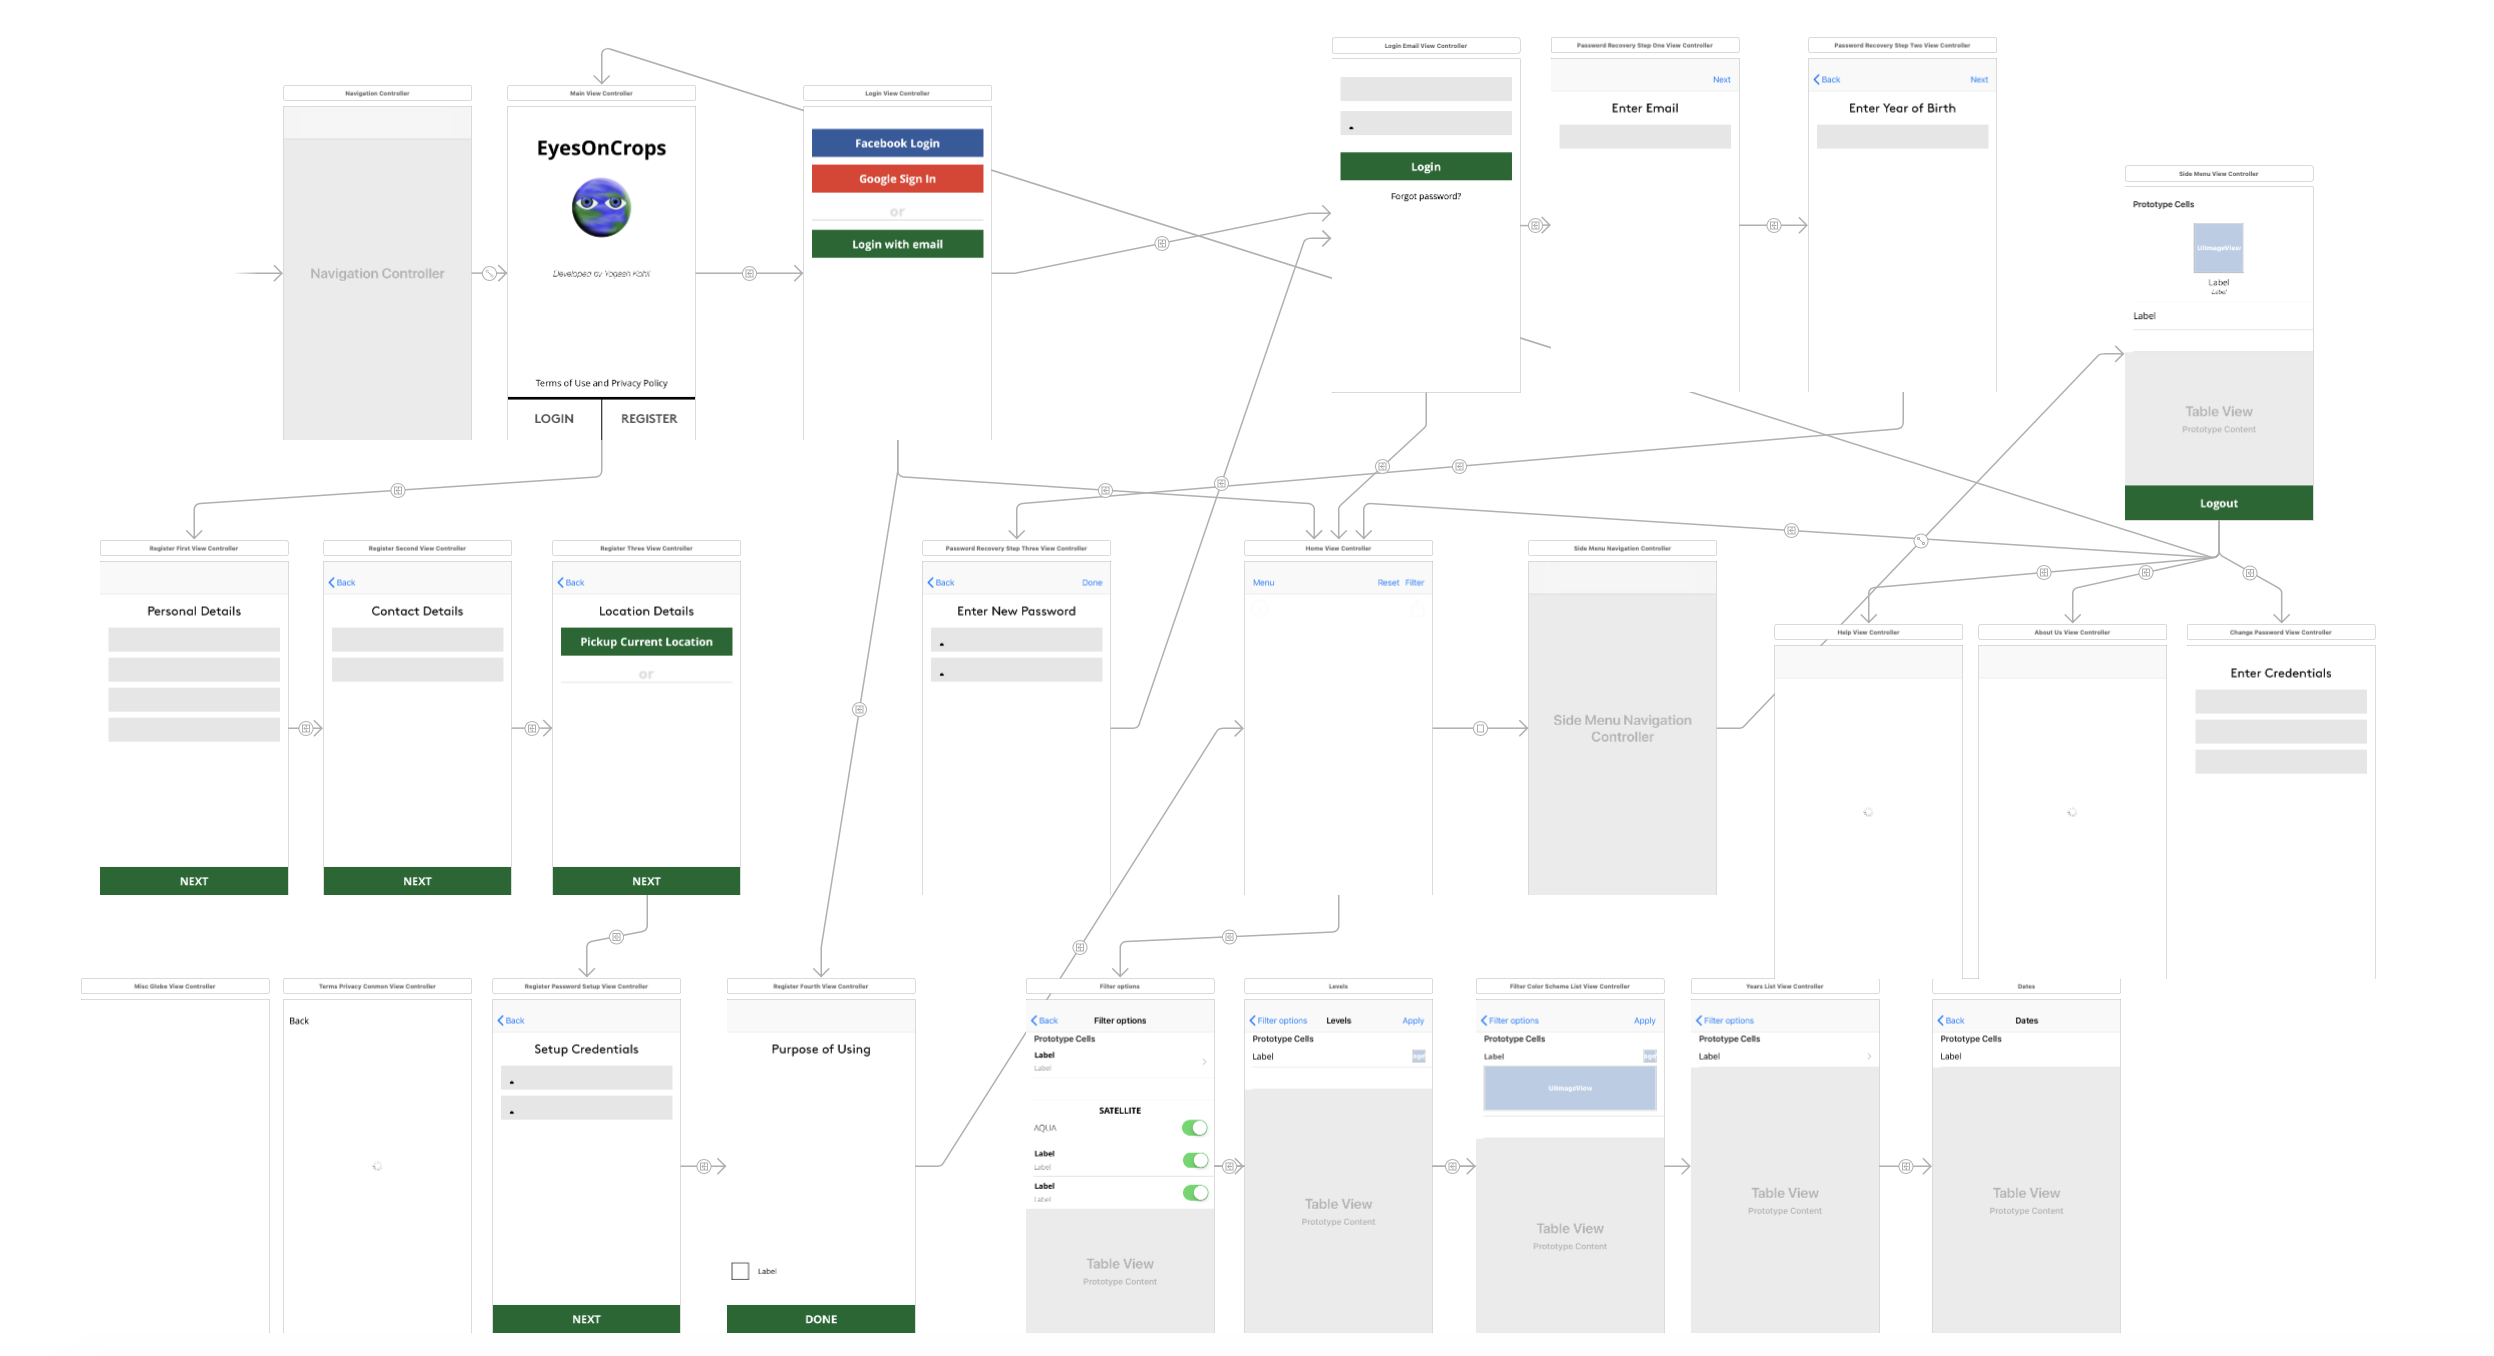
\includegraphics[width=\linewidth]{figures/ch4/storyboard_final.png}
    \caption{\label{fig:storyboard_final} Storyboard of the app}
\end{sidewaysfigure}
    
\subsection{Mobile App screens and their significance}

This part of the thesis focuses on the screens and their usage in the application. It explains all the screens categorized by the processes such as signup, login, home, slide out menu and filter.

\subsubsection{Sign-up via Email}

Sign up process is a one-time process which enables the user to enter the application out of the blue. It likewise gives the chance to include the client in the database for future logins and additionally for the record purpose. Sign up via email process consists of 5 screens which are listed below.

\begin{itemize}

    \item Personal details
    
    \begin{figure}[H]
            \centering
            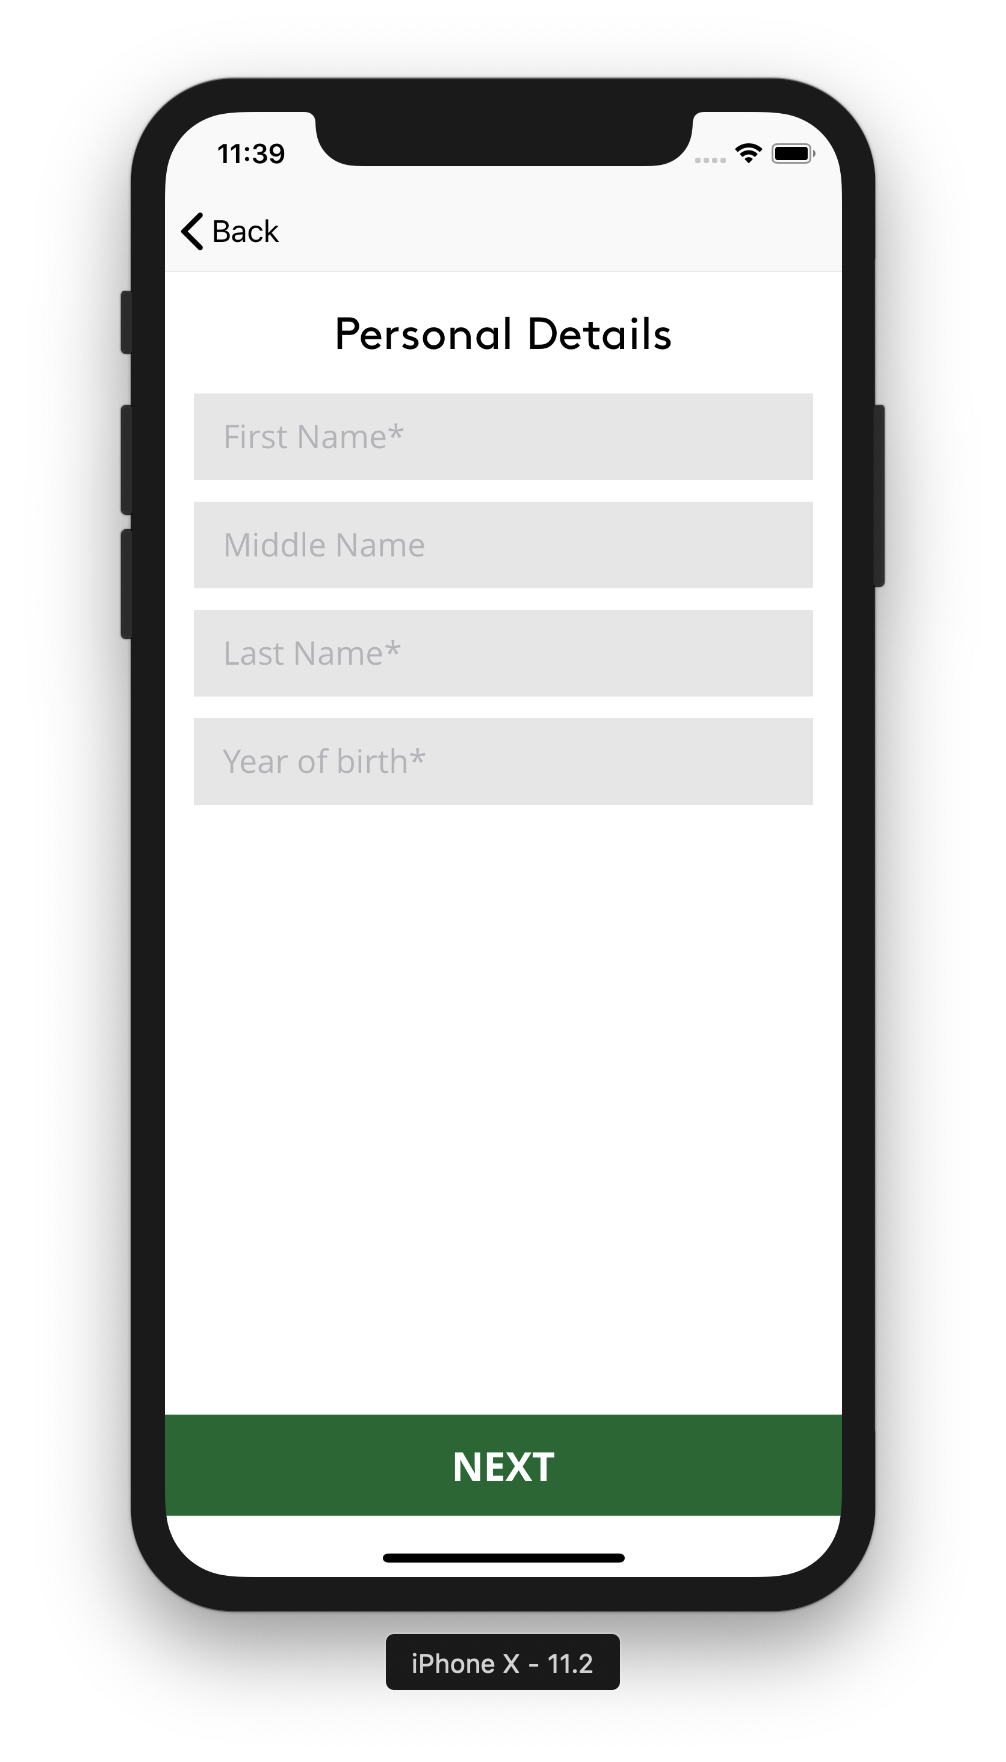
\includegraphics[width=0.25\linewidth]{figures/ch4/register_personal.png}
            \caption{\label{fig:register_personal_ch4} Register Part-I Personal detail screen}
    \end{figure}
    
    In Figure~\ref{fig:register_personal_ch4}, notice that mandatory fields are first name, last name and year of birth where middle name is kept as an optional (because not everyone has one). Year of birth has been taken from user to get the idea about what age group are using the application. UIPickerView is used for selection of year of birth, according to Apple's documentation, UIPickerView is a view that uses a spinning-wheel or slot-machine metaphor to show one or more sets of values. Figure~\ref{fig:pickerview} shows the image of the pickerview designed in the application.
    
    \begin{figure}[H]
            \centering
            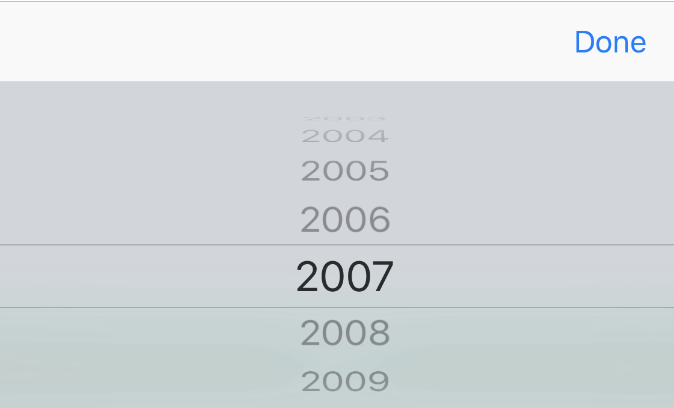
\includegraphics[width=0.25\linewidth]{figures/ch4/pickerview.png}
            \caption{\label{fig:pickerview} UIPickerView for year selection}
    \end{figure}
  
    \item Contact details
    
    \begin{figure}[H]
            \centering
            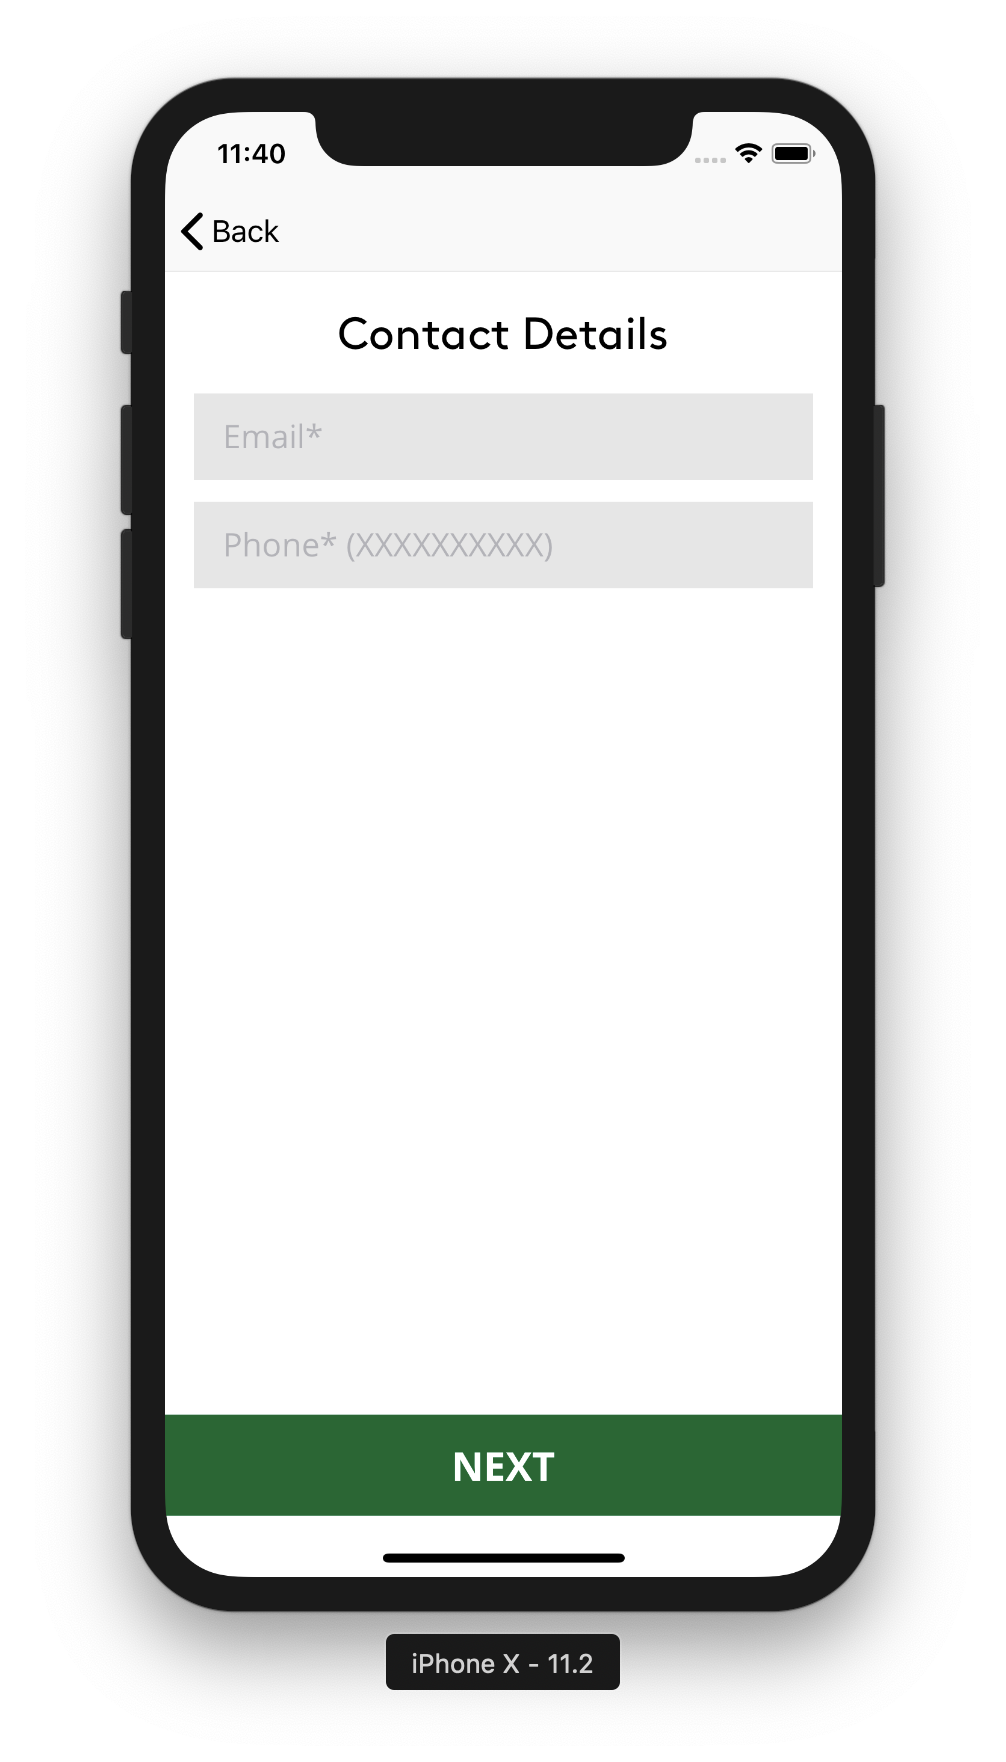
\includegraphics[width=0.25\linewidth]{figures/ch4/register_contact.png}
            \caption{\label{fig:register_contact_ch4} Register Part-II Contact detail screen}
    \end{figure}
    
    Figure~\ref{fig:register_contact_ch4} represents contact detail screen in which the fields i.e. email and phone are mandatory for record purpose and to provide login via email functionality. User with unique email and phone can register only once. It's good to note that both fields have been verified syntactically here.
    
    \item Location details
    
    \begin{figure}[H]
            \centering
            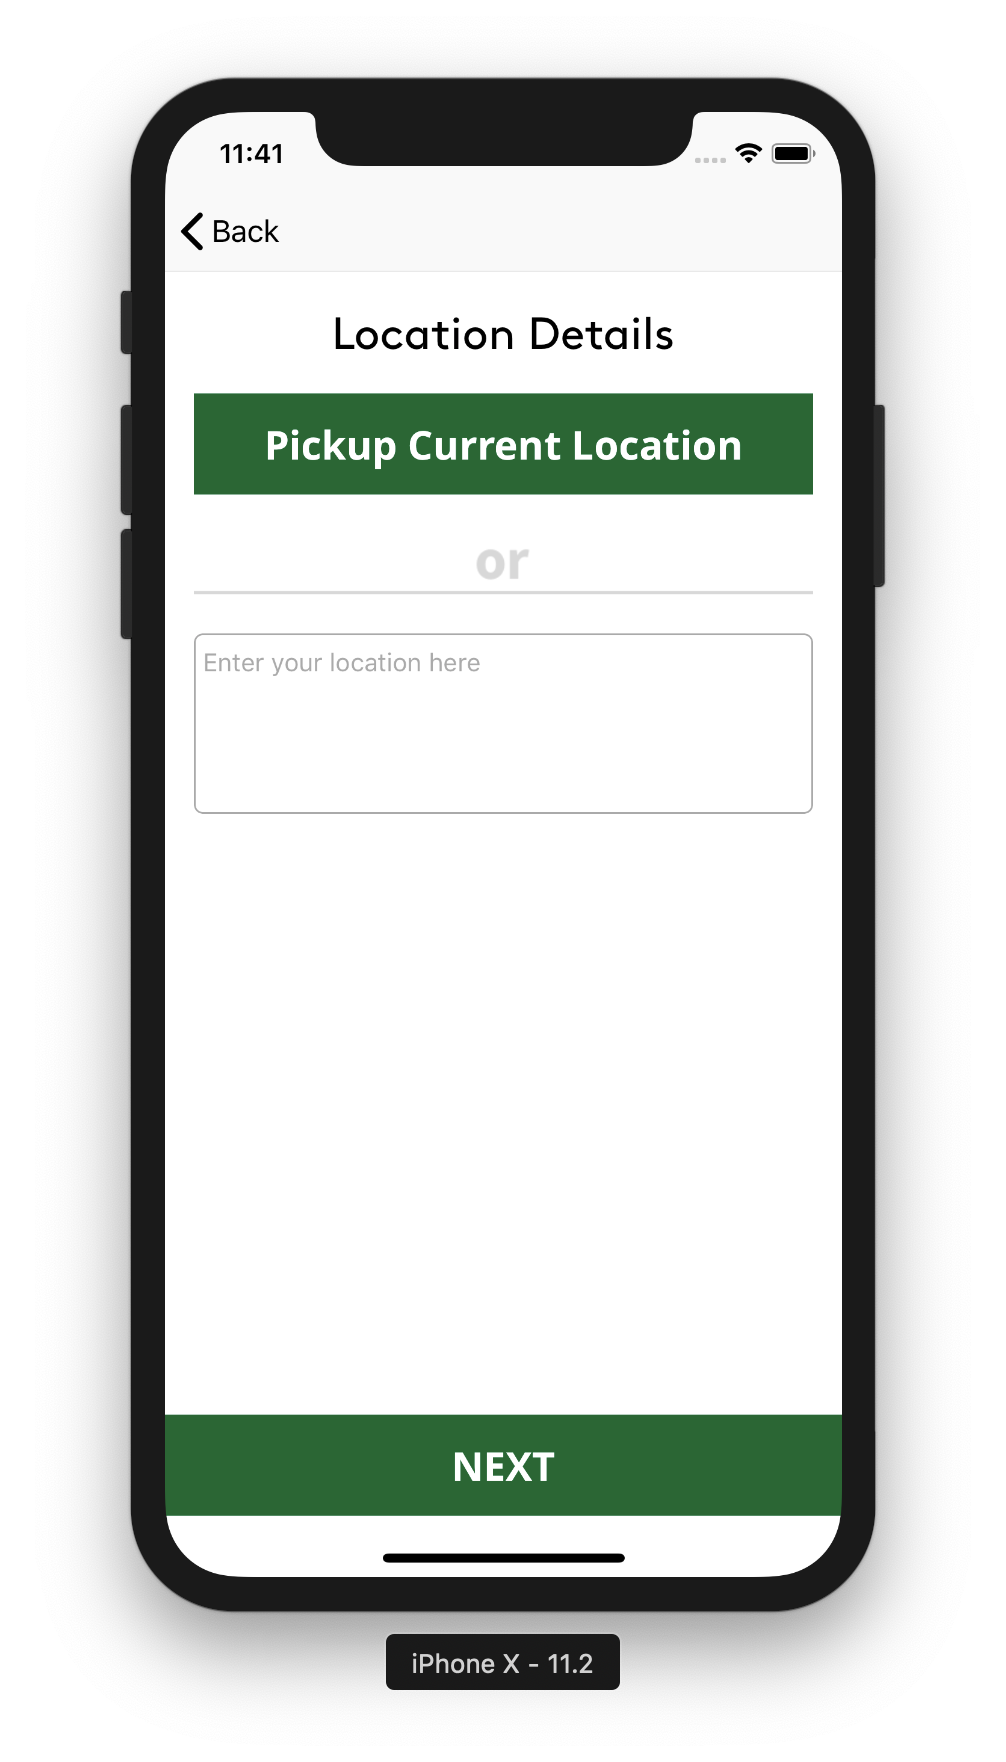
\includegraphics[width=0.25\linewidth]{figures/ch4/register_location.png}
            \caption{\label{fig:register_location_ch4} Register Part-III Location detail screen}
    \end{figure}
    
    The reason for having this screen is to get the location of the users that are using the application for analytics purpose. This screen makes use of Apple's Core Location framework which allows developers to obtain current geographic location of the device. In this screen, user has two choices for entering the location, the user can enter the area physically or can simply tap on pickup current area which will eventually get the present location and display it in text area. Despite everything the user can still alter the area if needed.
  
    \item Setup Credentials
    
    \begin{figure}[H]
            \centering
            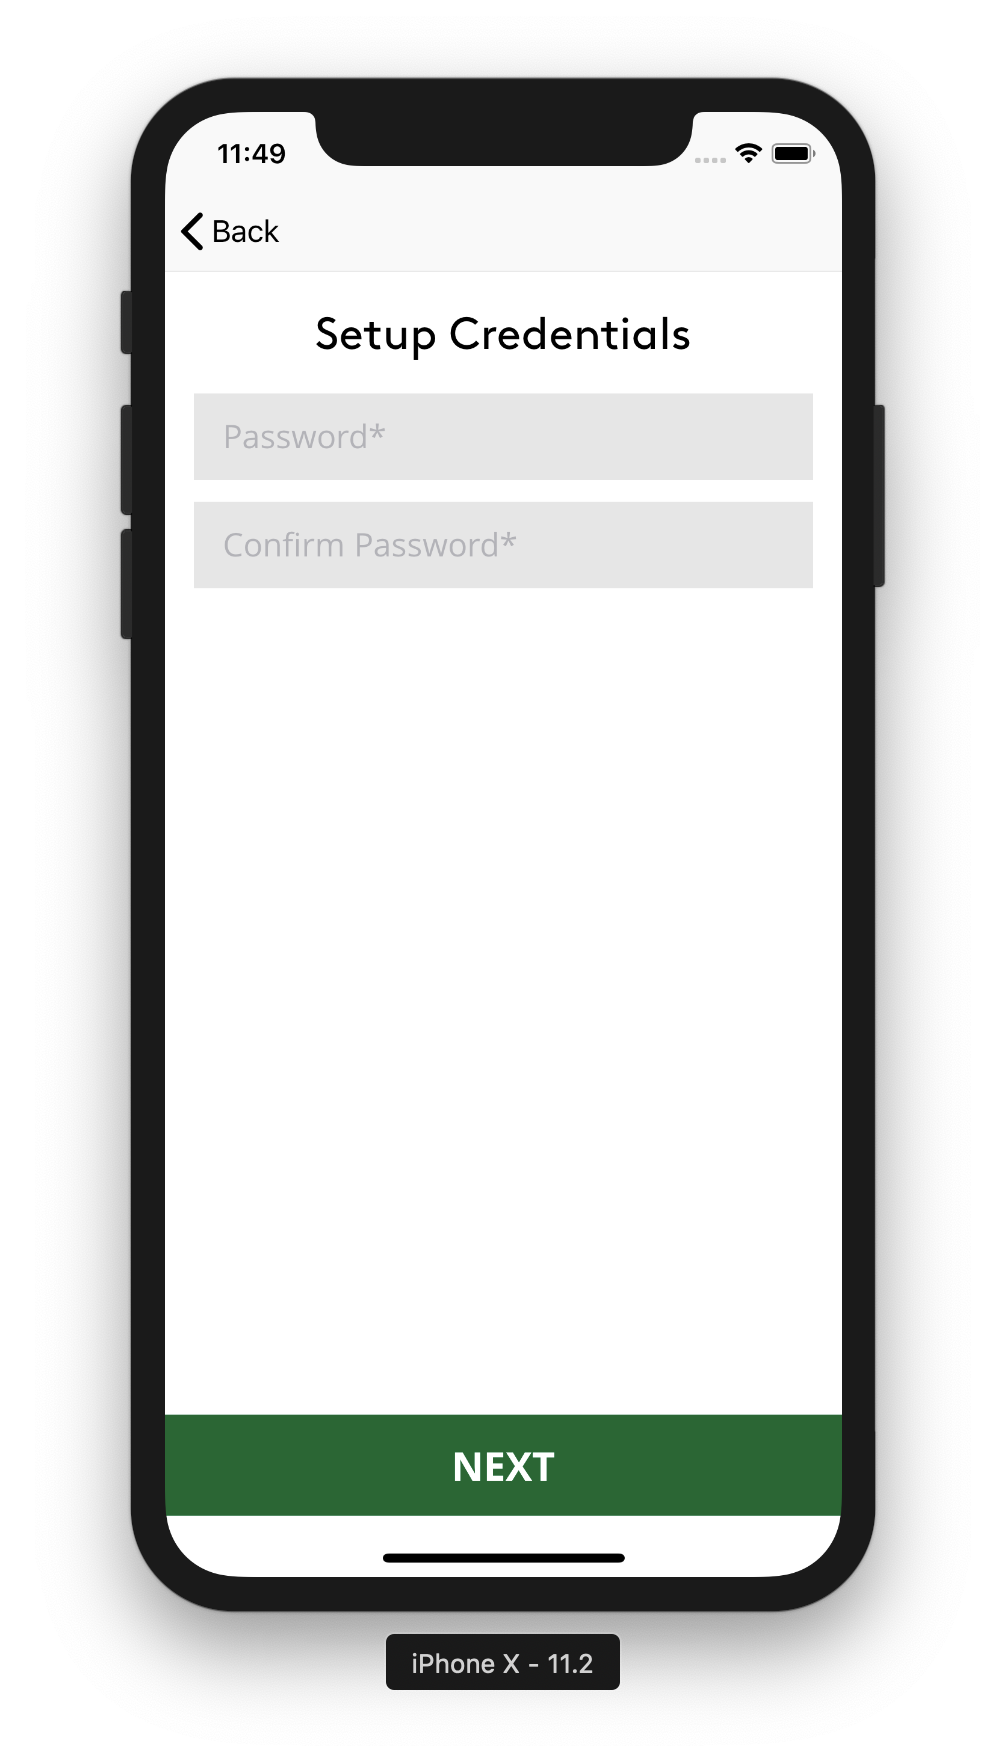
\includegraphics[width=0.25\linewidth]{figures/ch4/credentials_setup.png}
            \caption{\label{fig:credentials_setup_ch4} Register Part-IV Credentials setup screen}
    \end{figure}
    
    As shown in Figure~\ref{fig:credentials_setup_ch4} , it allows the user to setup password for a secure login. Important thing here is that minimum length of password is set to 6 digits.
   
    \item Purpose of using the app
    
     \begin{figure}[H]
            \centering
            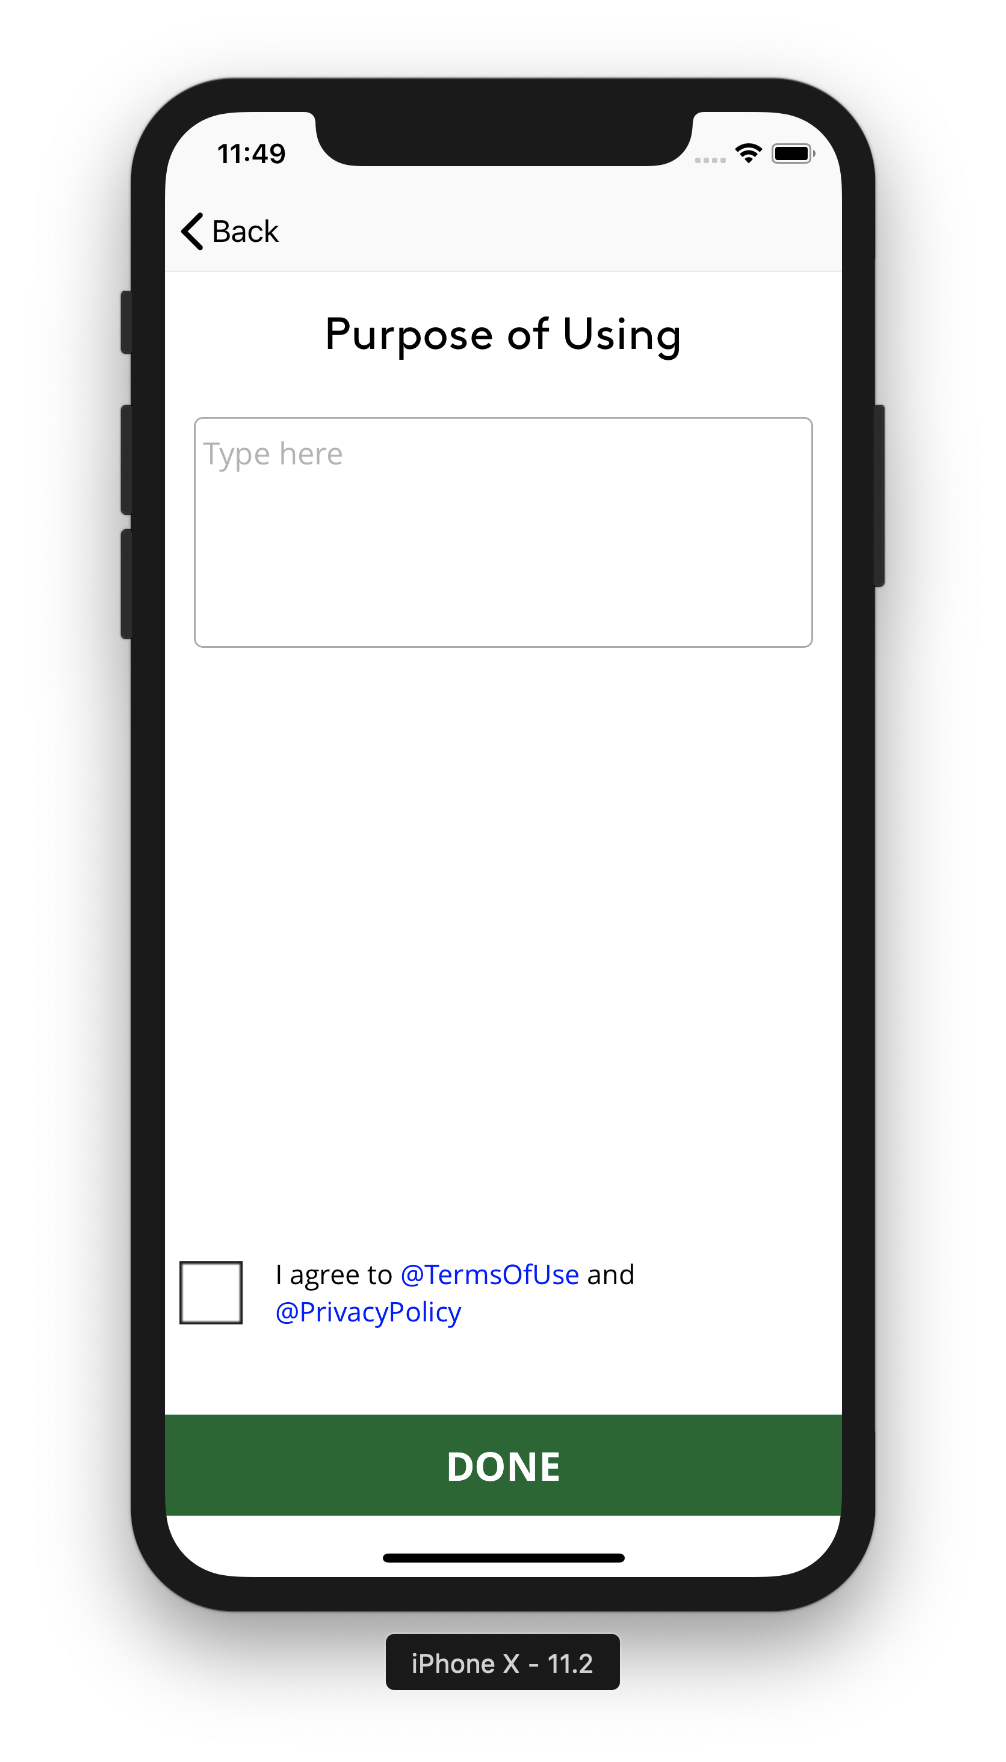
\includegraphics[width=0.25\linewidth]{figures/ch4/purpose_app.png}
            \caption{\label{fig:purpose_app_ch4} Register Part-V Purpose of using the app screen}
    \end{figure}
    
    This screen is really important since it shows how and why people wants to use this app. Moreover, it has an additional check mark for privacy policy and terms of use to which every user must agree before going further.
   
\end{itemize}

\subsubsection{Login process}

Users can login into the app via certain ways which are mentioned below.

\begin{itemize}
    \item Social Login
    
    Login functionality has been further divided into social platforms which are explained below.
    
    \begin{itemize}
        \item Facebook Login
        
       The Facebook \gls{sdk} for \gls{iOS} provides developers to integrate a plugin, which allows users to log into their Facebook accounts. Figure~\ref{fig:facebook_part_1} shows the pop up alert which shows up after tapping on Facebook login button and Figure~\ref{fig:facebook_part_2} shows the screens when user opts for Facebook log in after clicking "continue" in Figure~\ref{fig:facebook_part_1}.
       
      \begin{figure}[!htb]
        \begin{minipage}{0.5\textwidth}
            \centering
            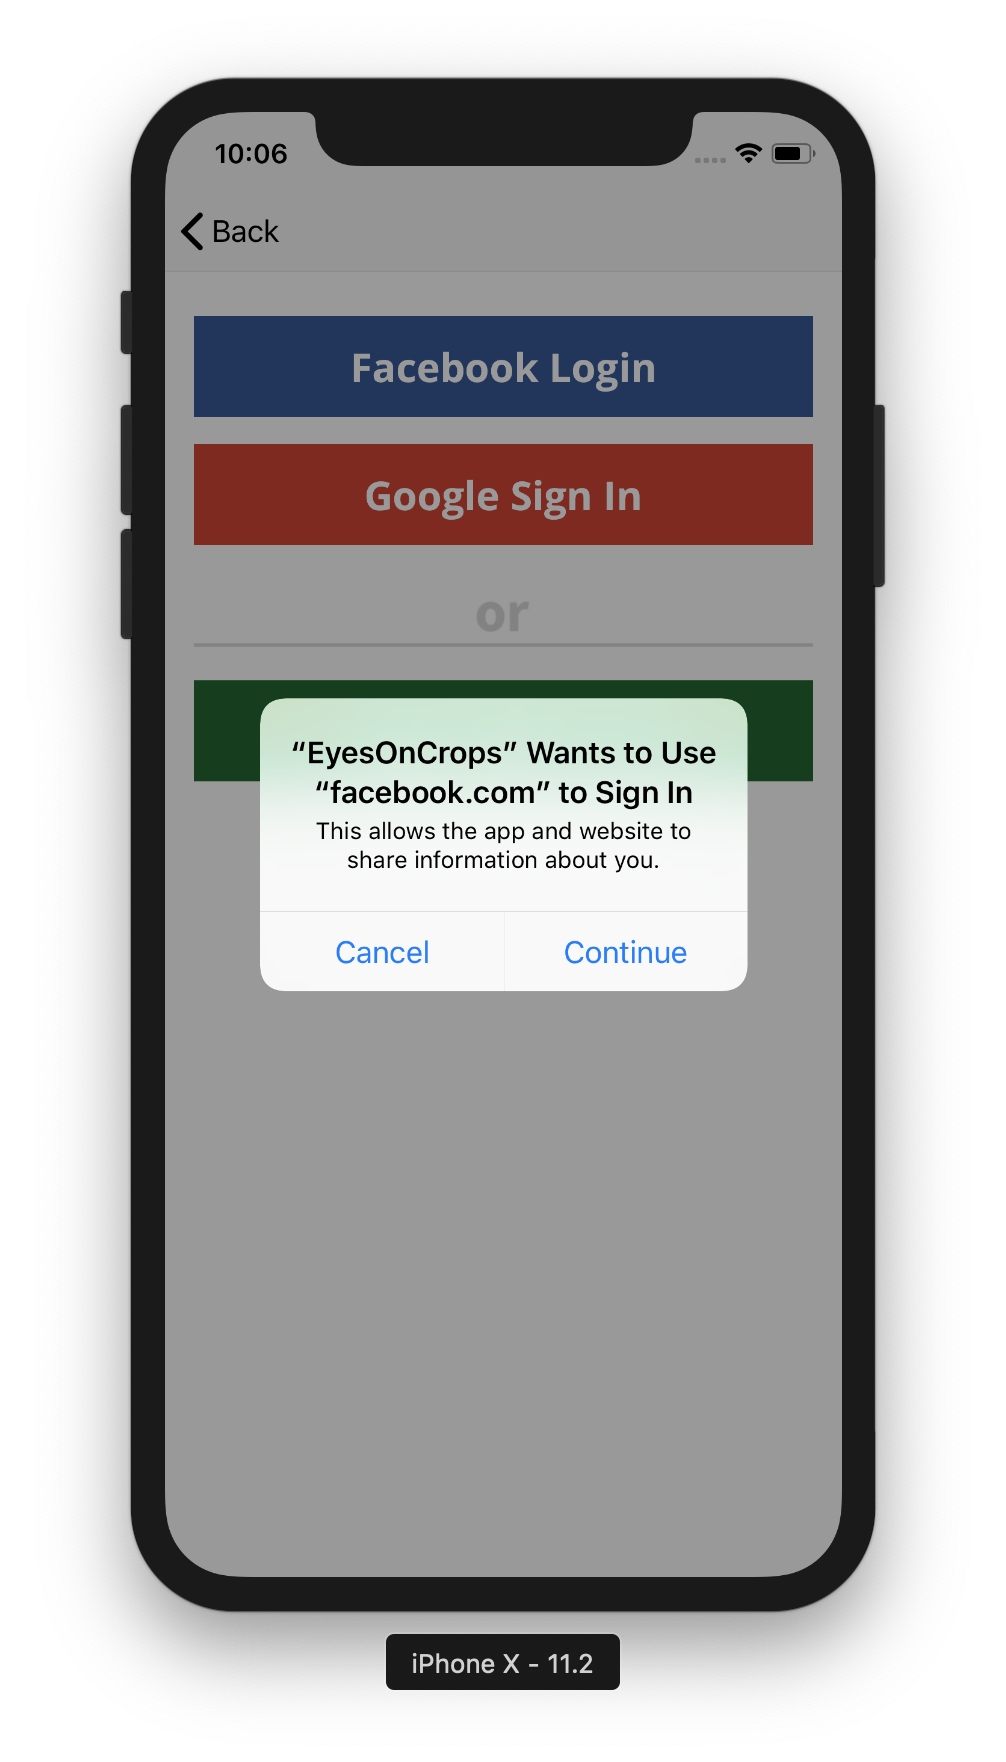
\includegraphics[width=0.5\linewidth]{figures/ch4/facebook_1.png}
            \caption{Facebook log in Part-I}\label{fig:facebook_part_1}
        \end{minipage}\hfill
        \begin{minipage}{0.5\textwidth}
            \centering
            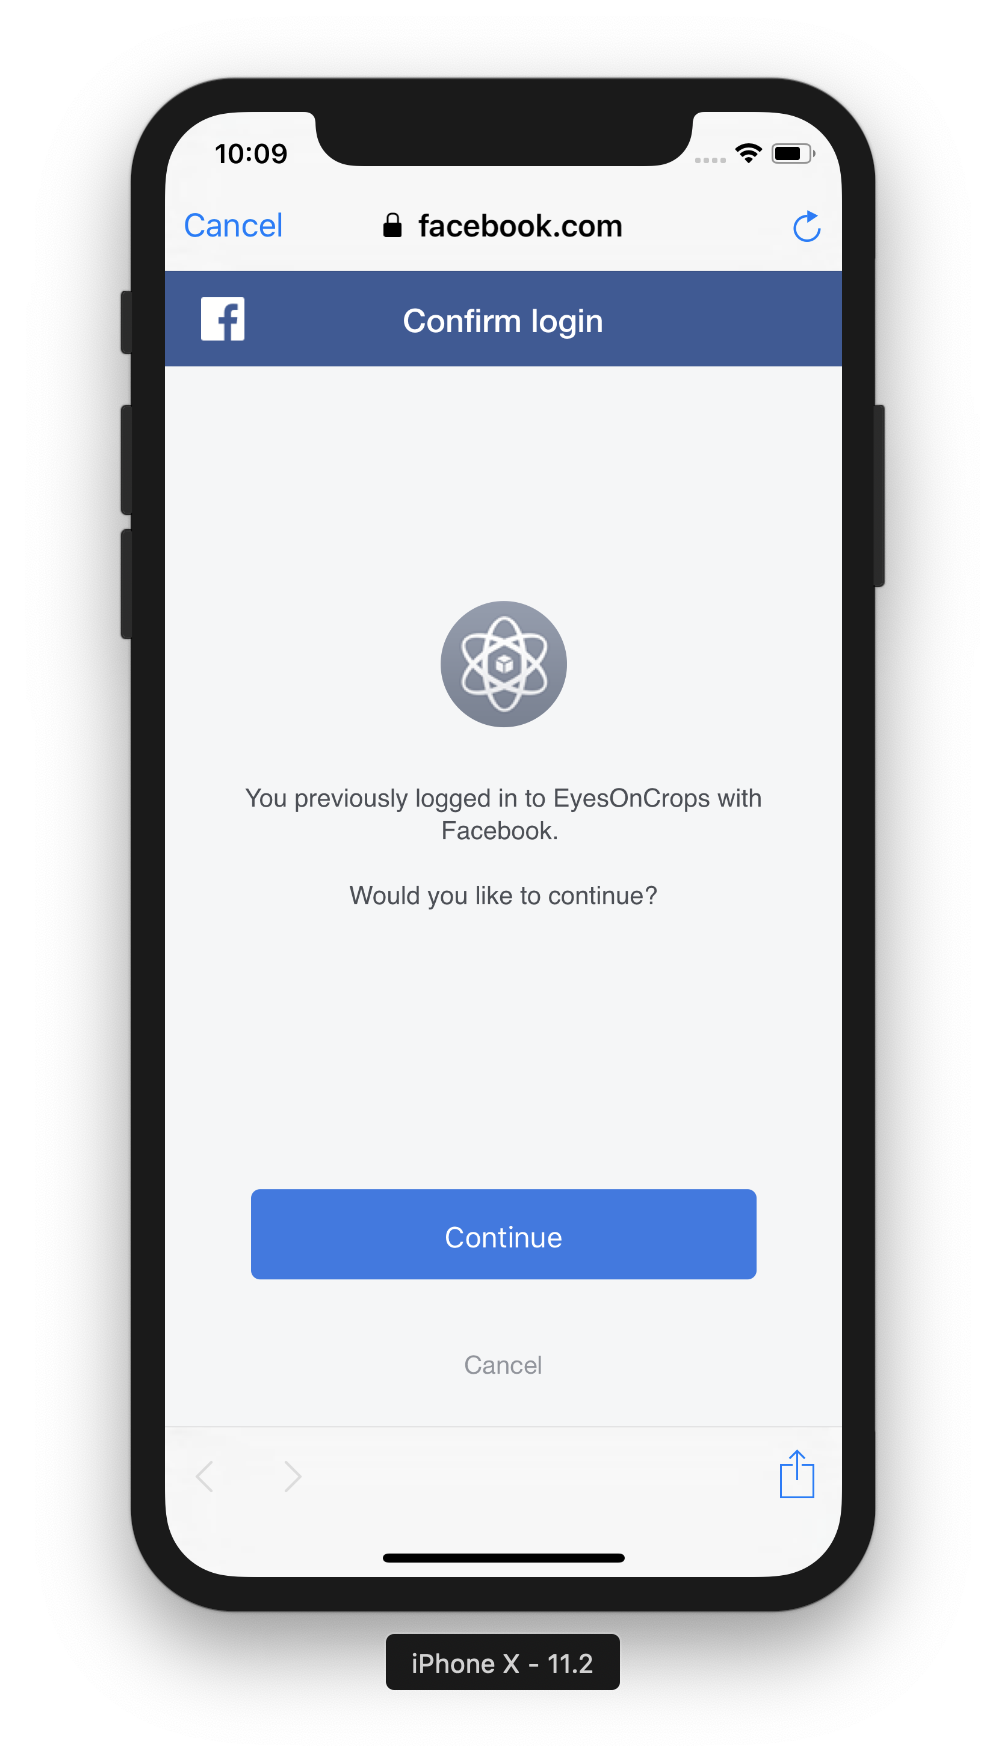
\includegraphics[width=0.5\linewidth]{figures/ch4/facebook_2.png}
            \caption{Facebook log in Part-II}\label{fig:facebook_part_2}
        \end{minipage}
    \end{figure}
    
        Figure~\ref{fig:facebook_part_2} shows that the user doesn't have to enter his/her Facebook id and password every time, it's a one time process, the \gls{sdk} helps developers to remember the credentials previously used.
        
      
        \item Google Sign in
        
        User can also login through their Gmail account by tapping on Google sign in button, if they don't have Facebook account or vice-verse as shown in Figure~\ref{fig:google_part_1}. Google's \gls{api} for sign-in has been implemented to create this functionality in the app. Figure~\ref{fig:google_part_1} and ~\ref{fig:google_part_2} shows Google \gls{sdk} sign in process. \\
        
        \begin{figure}[!htb]
        \begin{minipage}{0.5\textwidth}
            \centering
            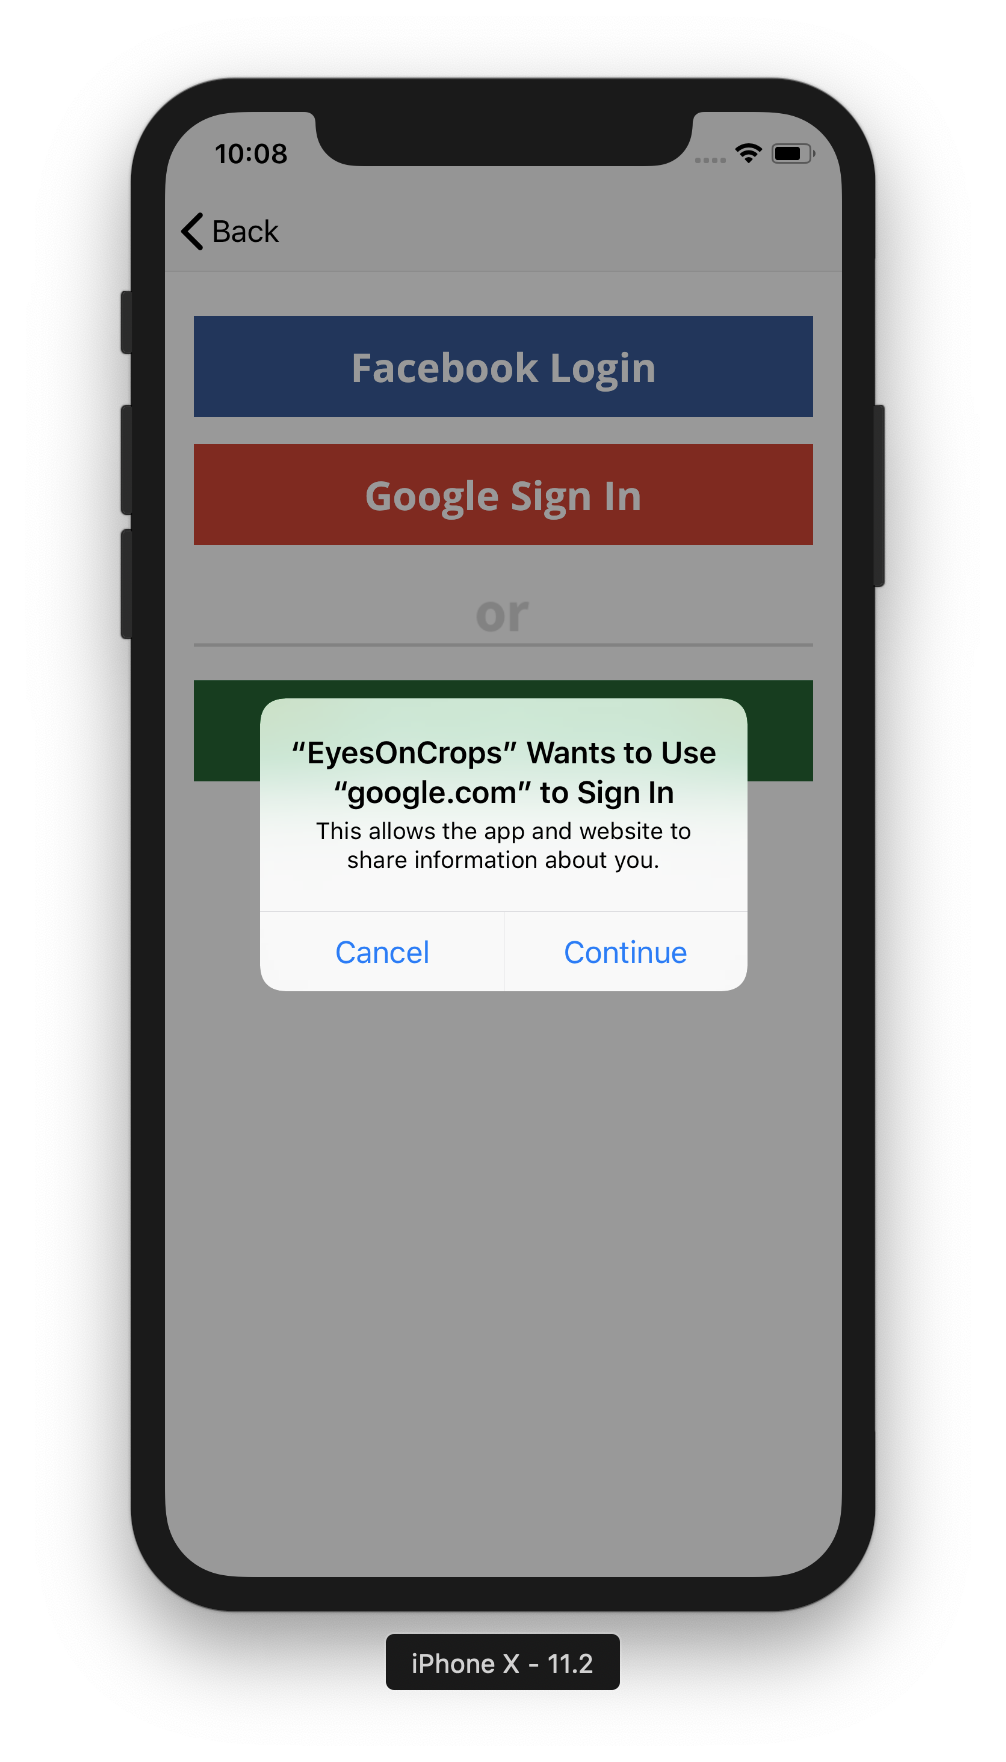
\includegraphics[width=0.5\linewidth]{figures/ch4/google_1.png}
            \caption{Google sign in Part-I}\label{fig:google_part_1}
        \end{minipage}\hfill
        \begin{minipage}{0.5\textwidth}
            \centering
            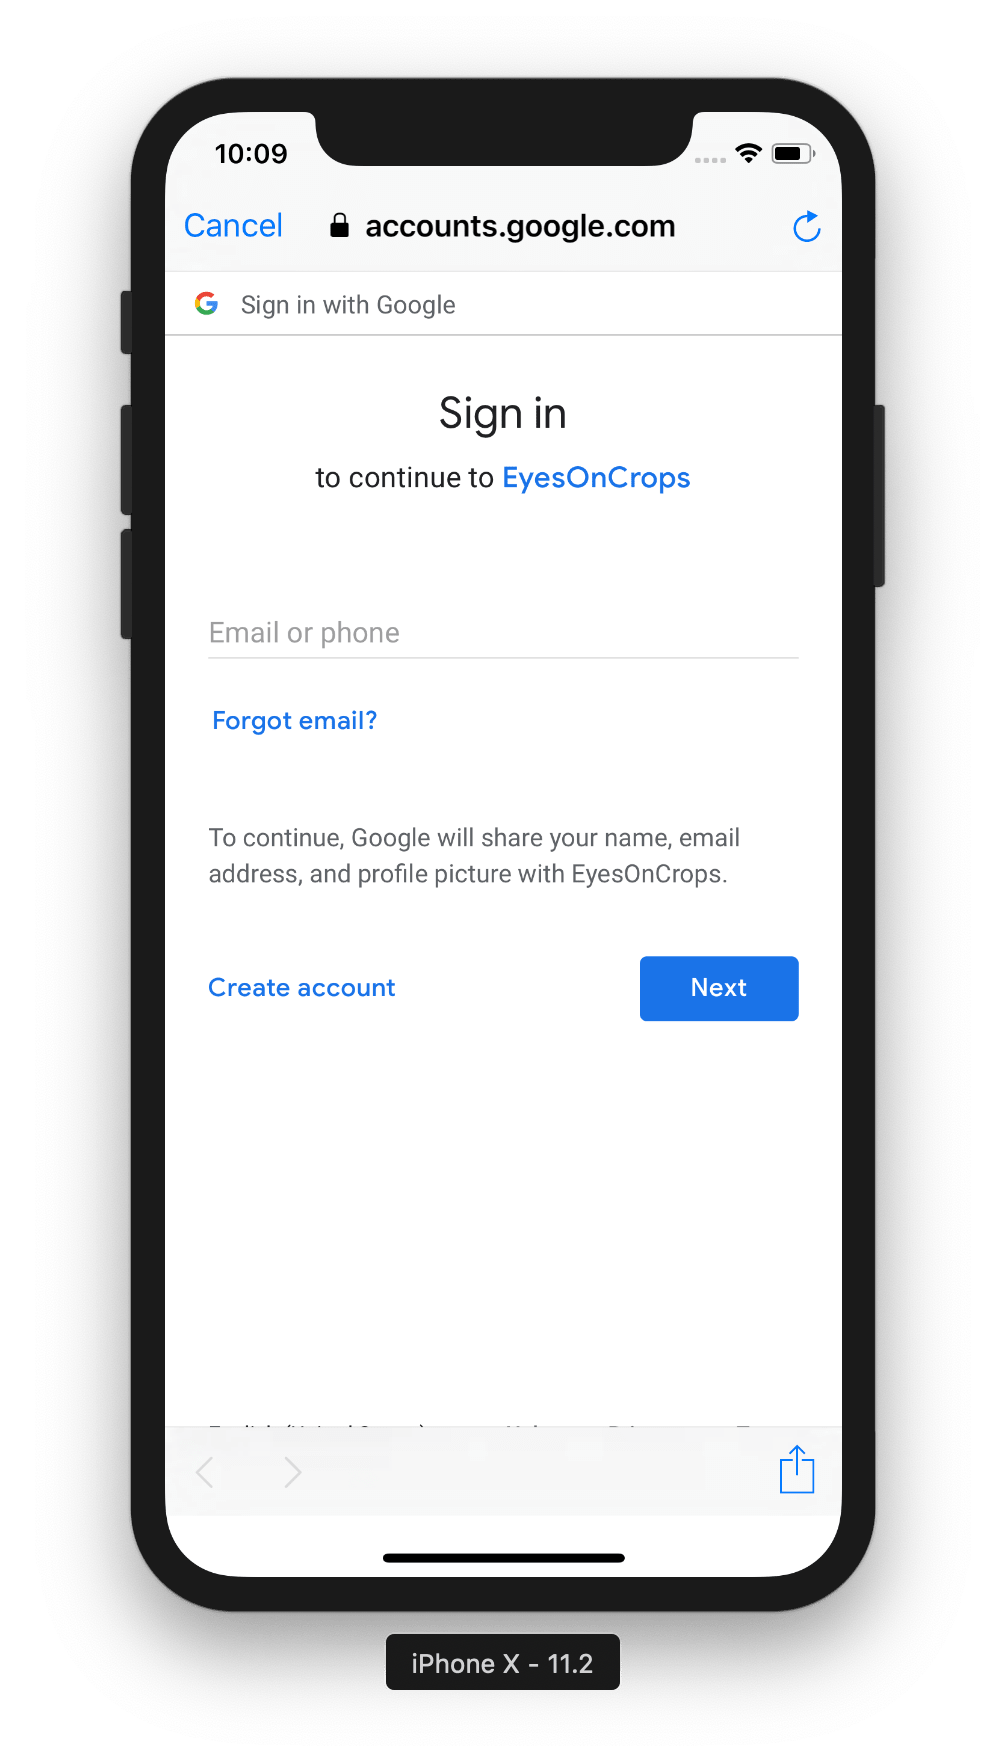
\includegraphics[width=0.5\linewidth]{figures/ch4/google_2.png}
            \caption{Google sign in Part-II}\label{fig:google_part_2}
        \end{minipage}
    \end{figure}
        
    \end{itemize}
 
    \item Login via email
    
    Those users who have registered via email can utilize the functionality of log in via email. They will be required to enter valid email and password to do so. Figure~\ref{fig:login_email_ch4} shows the login with email screen.
    
    \begin{figure}[H]
            \centering
            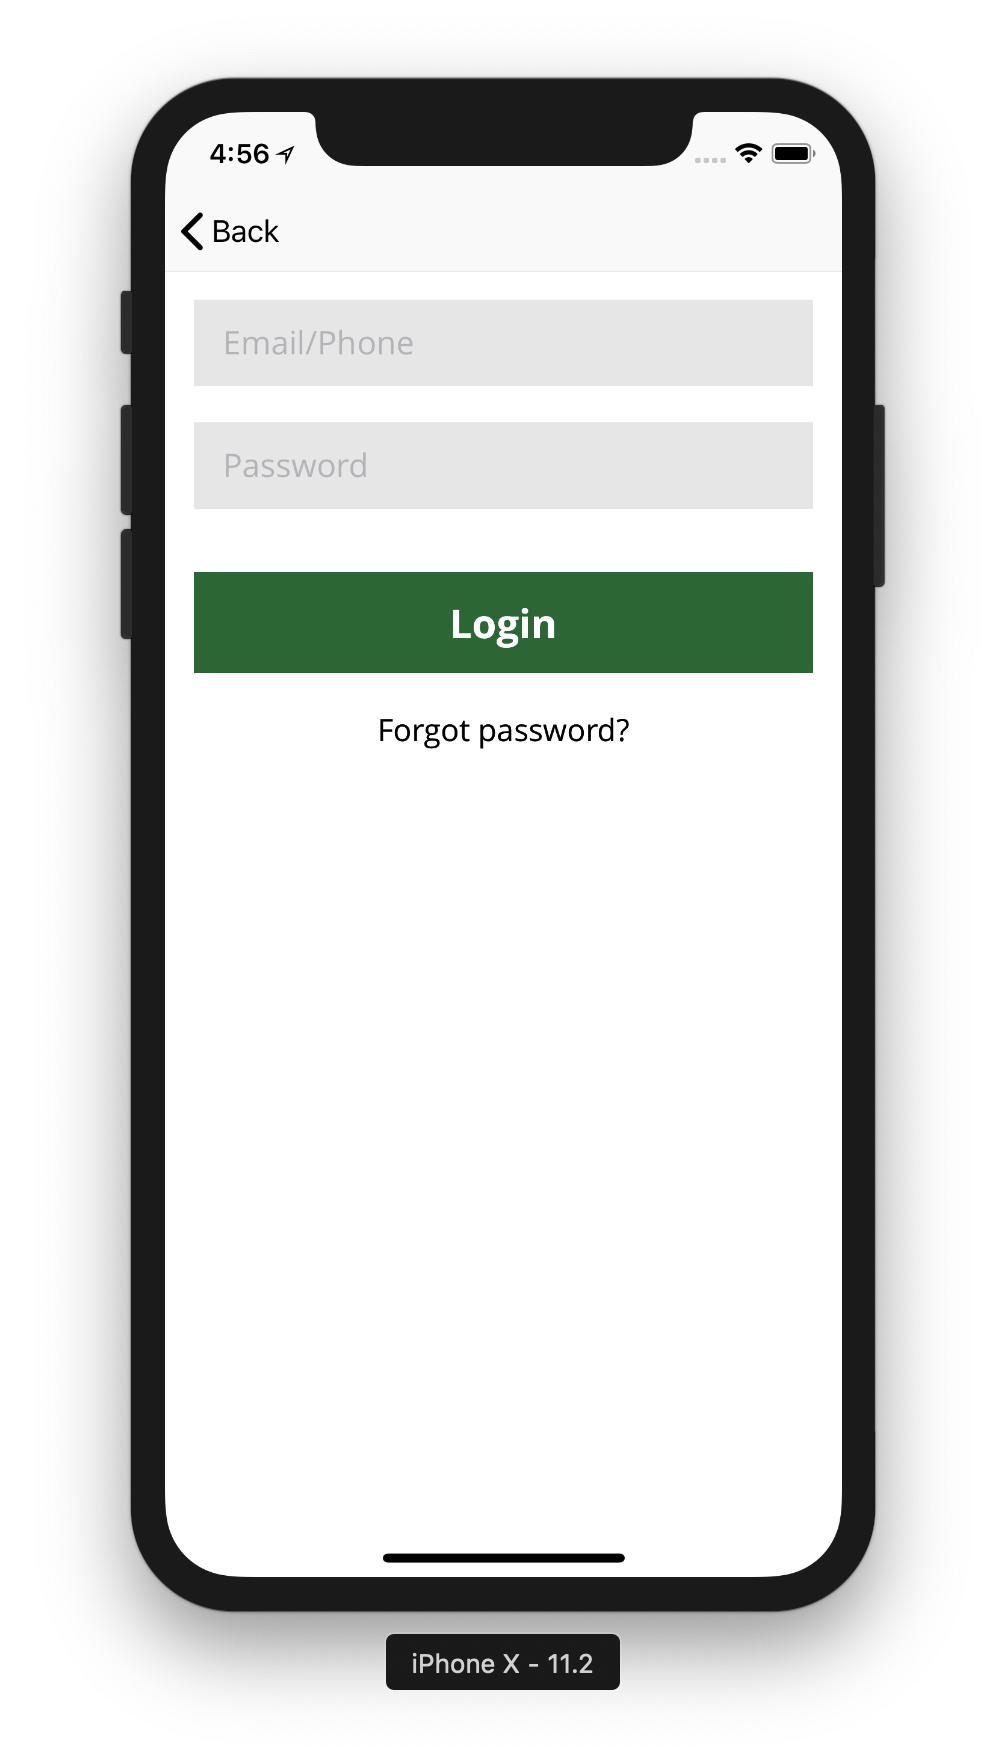
\includegraphics[width=0.25\linewidth]{figures/ch4/login_email.png}
            \caption{\label{fig:login_email_ch4} Login via email}
    \end{figure}
    
    Also, if users happen to forget their password, they can tap on forgot password button as shown in Figure~\ref{fig:pass_recovery_1} and follow the certain steps to change his password. \textbf{Password recovery} screens and their significance are explained below. 
    
    \newpage
    
    \begin{itemize}
        \item Email verification screen
        
        \begin{figure}[H]
            \centering
            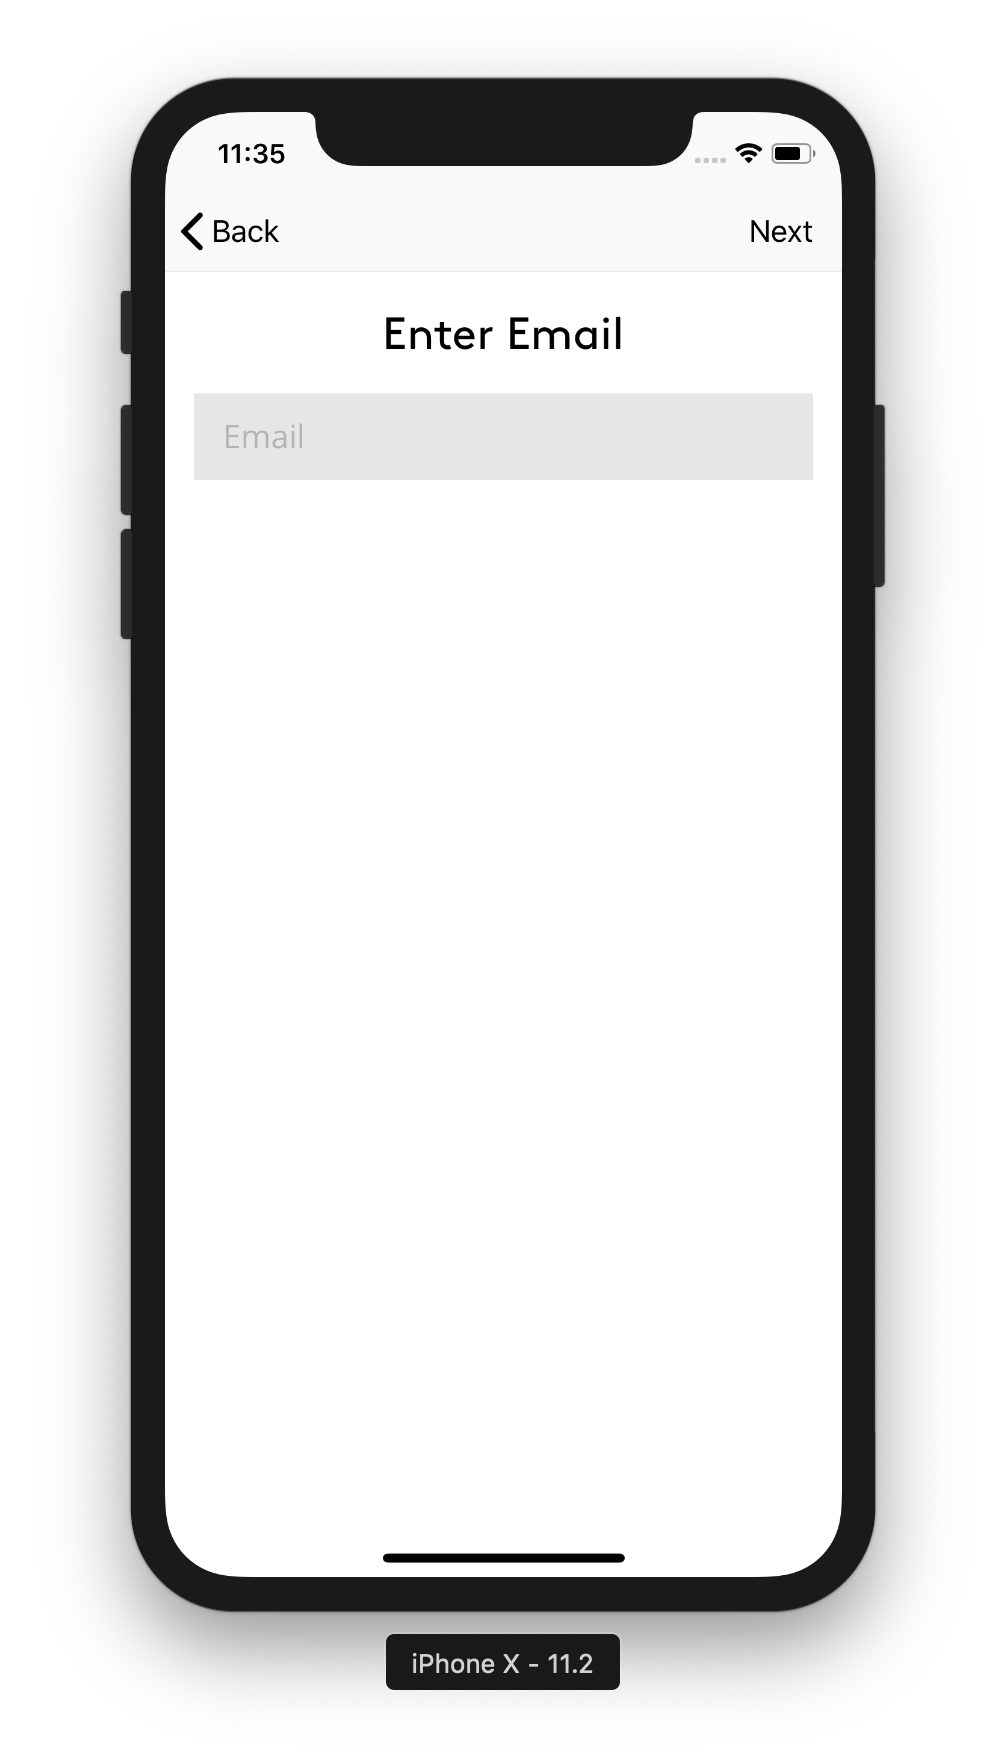
\includegraphics[width=0.25\linewidth]{figures/ch4/pass_recovery_1.png}
            \caption{\label{fig:pass_recovery_1} Password Recovery Part-I - Email verification}
        \end{figure}
    
    First part of the password recovery is to check if the user exist with the email entered in the Figure~\ref{fig:pass_recovery_1}. If yes, then take them to next screen else show an alert saying that record does not exist with this email.
    
     \item Year of birth verification screen
        
        \begin{figure}[H]
            \centering
            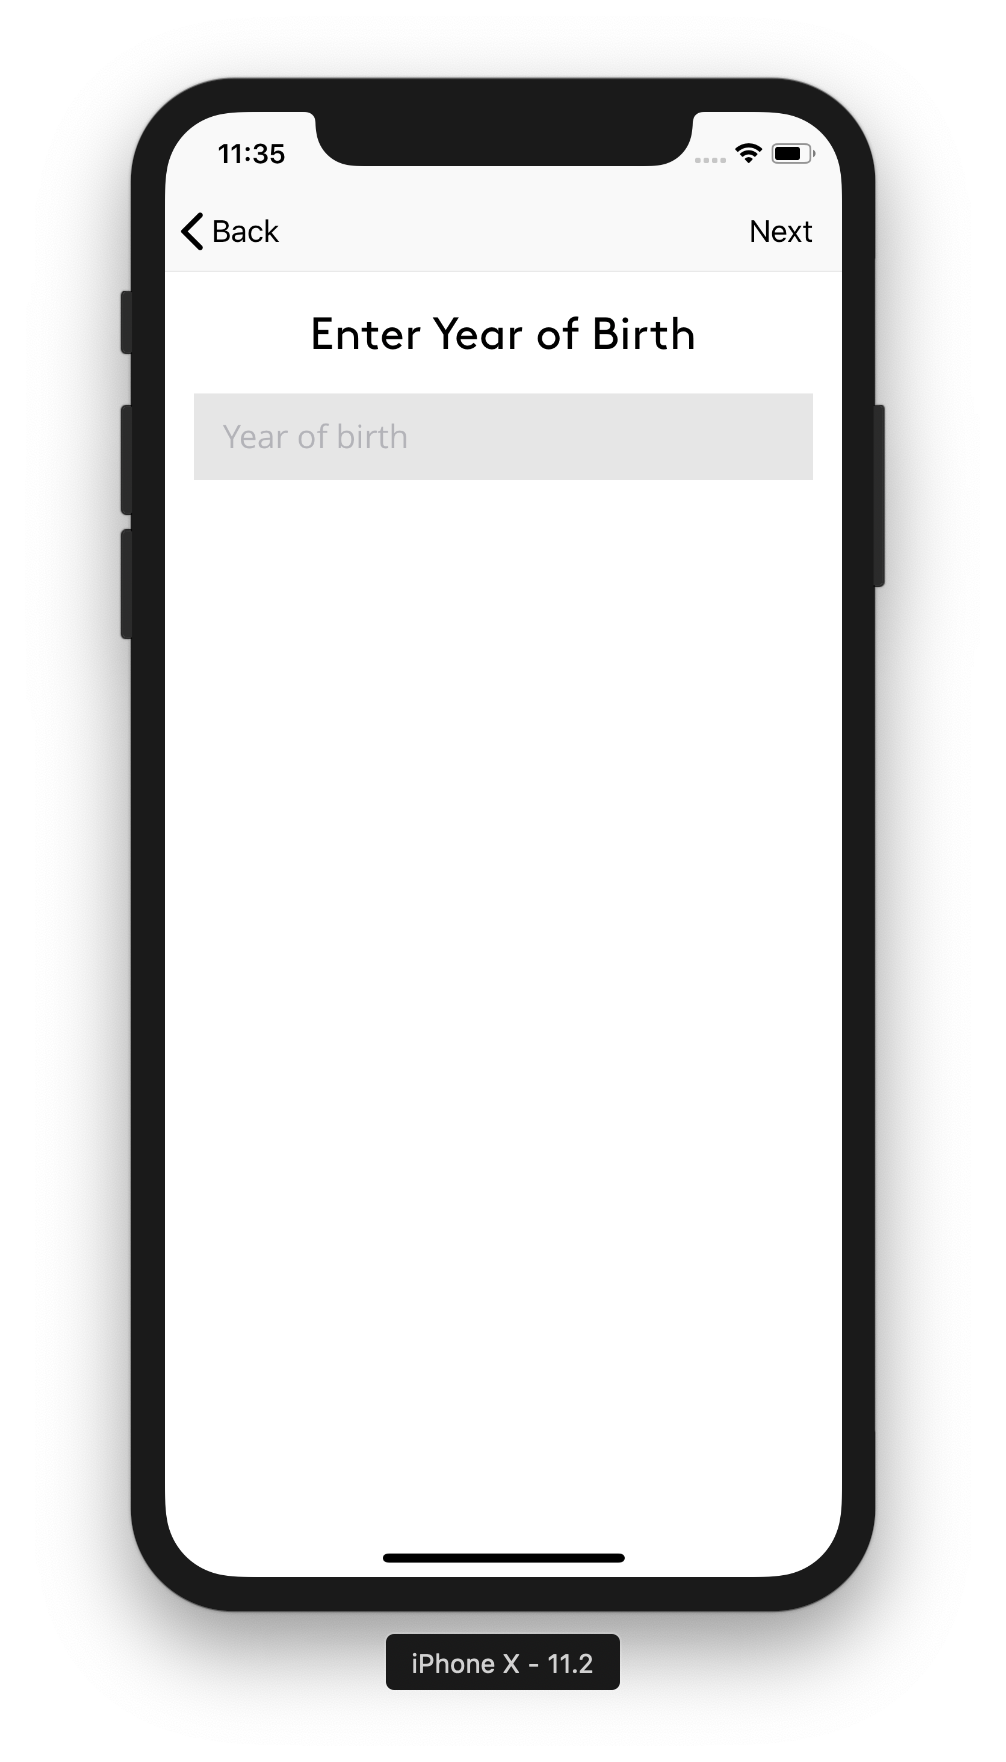
\includegraphics[width=0.25\linewidth]{figures/ch4/pass_recovery_2.png}
            \caption{\label{fig:pass_recovery_2} Password Recovery Part-II - Year of birth verification}
    \end{figure}
    
    This screen is to make this process more secure by asking users year of birth. It must match the year of birth they entered in registering via email process. If this match, then user is allowed to change the password.
 
     \item Change credentials screen
        
        \begin{figure}[H]
            \centering
            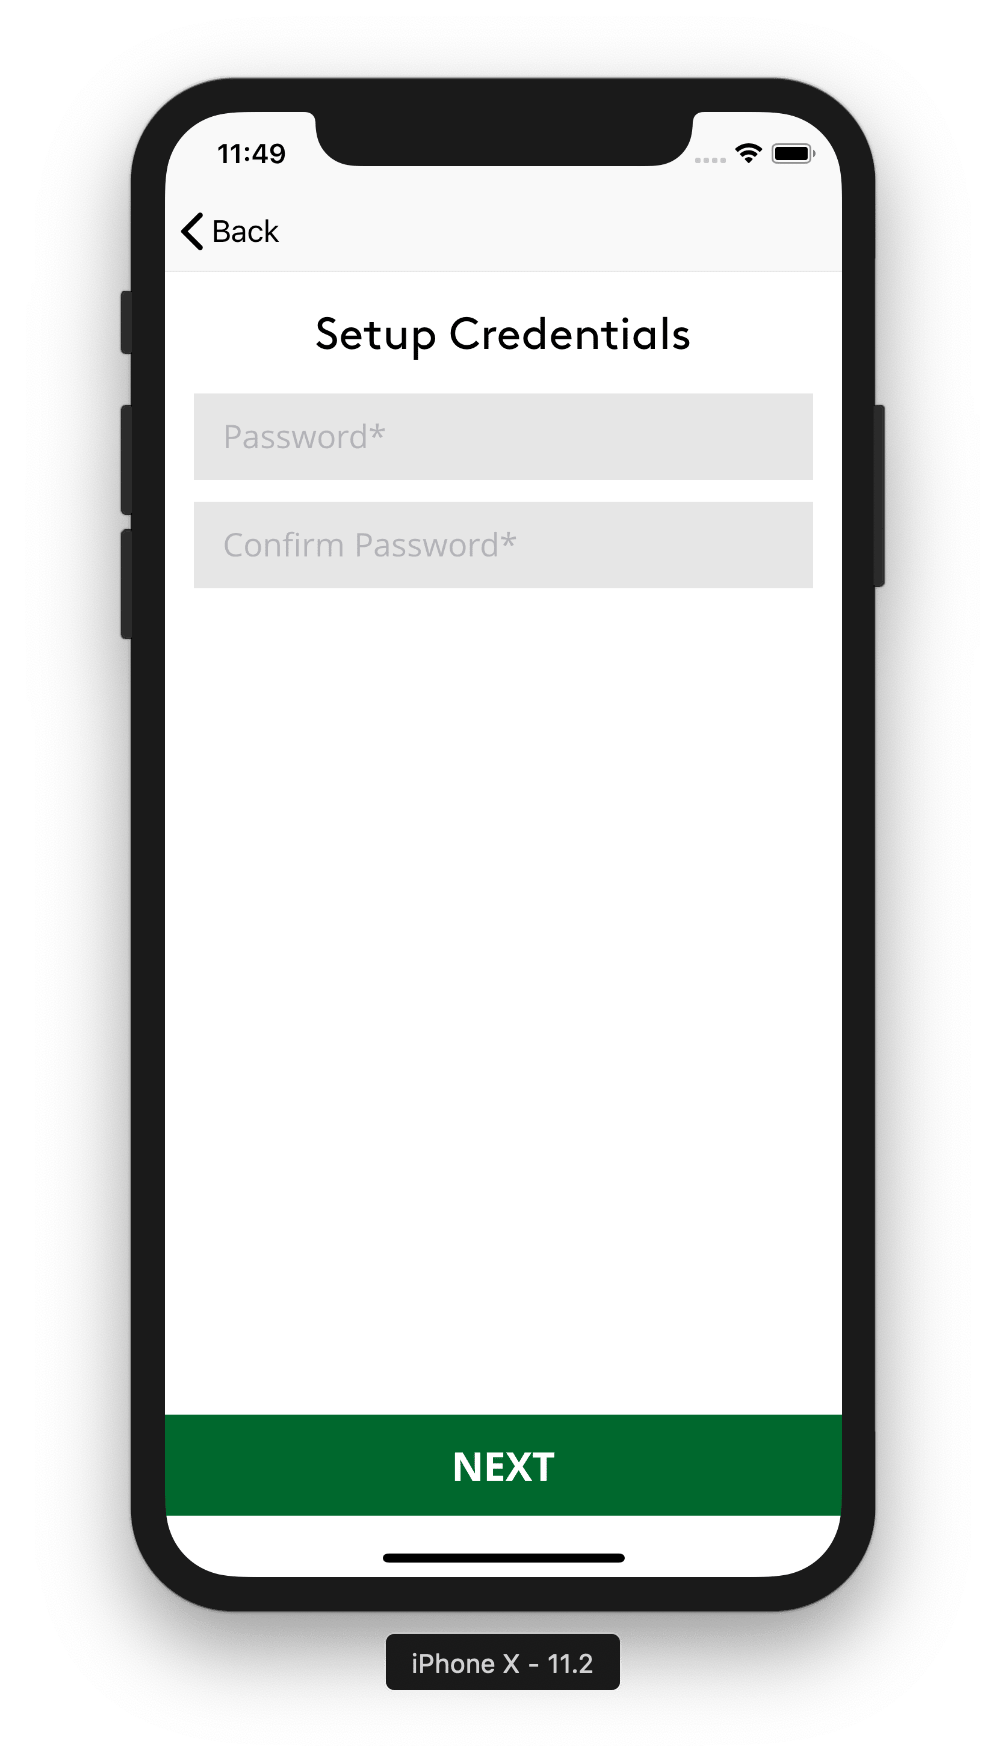
\includegraphics[width=0.25\linewidth]{figures/ch4/pass_recovery_3.png}
            \caption{\label{fig:pass_recovery_3} Password Recovery Part-III- Change credentials screen}
        \end{figure}
    
    Screen shown in Figure~\ref{fig:pass_recovery_3}  enables users to create new password.
    
    \end{itemize}
    
\end{itemize}

\subsubsection{Home screen}

This is an essential part of any application. In a context of mobile applications, it's the main screen from which users interact with the application. Home screen has two modes which are mentioned below.

    \begin{figure}[!htb]
        \begin{minipage}{0.5\textwidth}
            \centering
            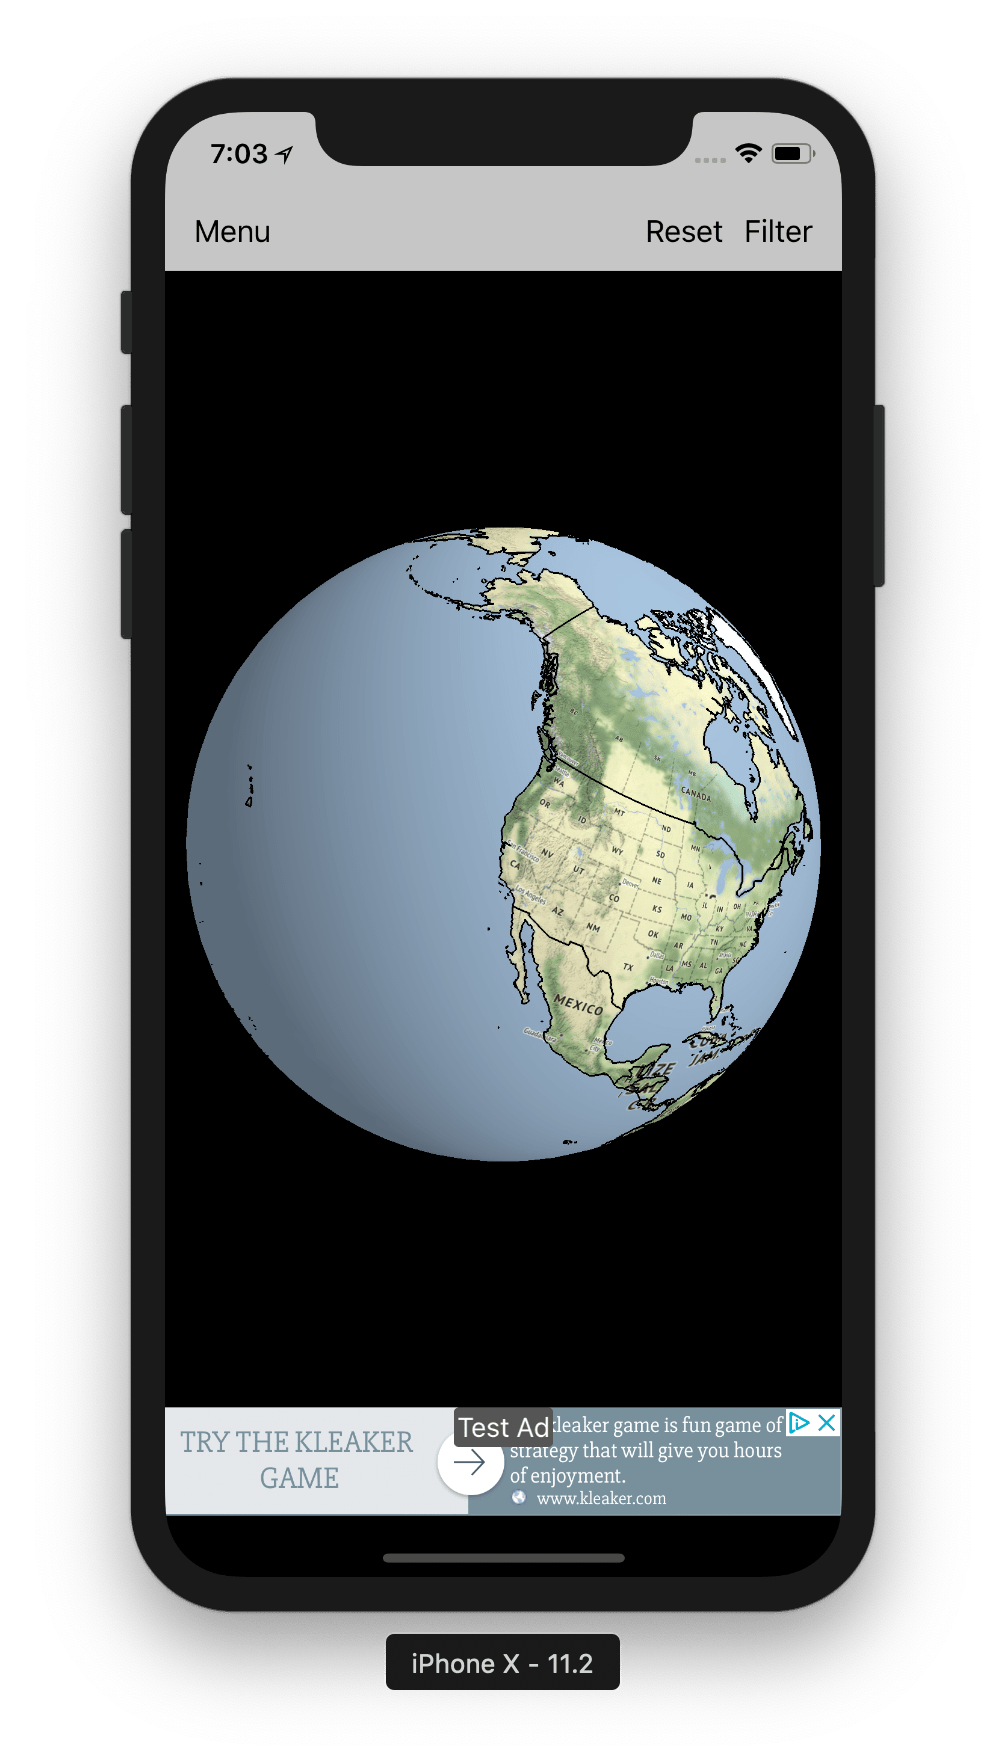
\includegraphics[width=0.5\linewidth]{figures/ch4/home_globe.png}
            \caption{Globe view}\label{fig:home_globe_mode}
        \end{minipage}\hfill
        \begin{minipage}{0.5\textwidth}
            \centering
            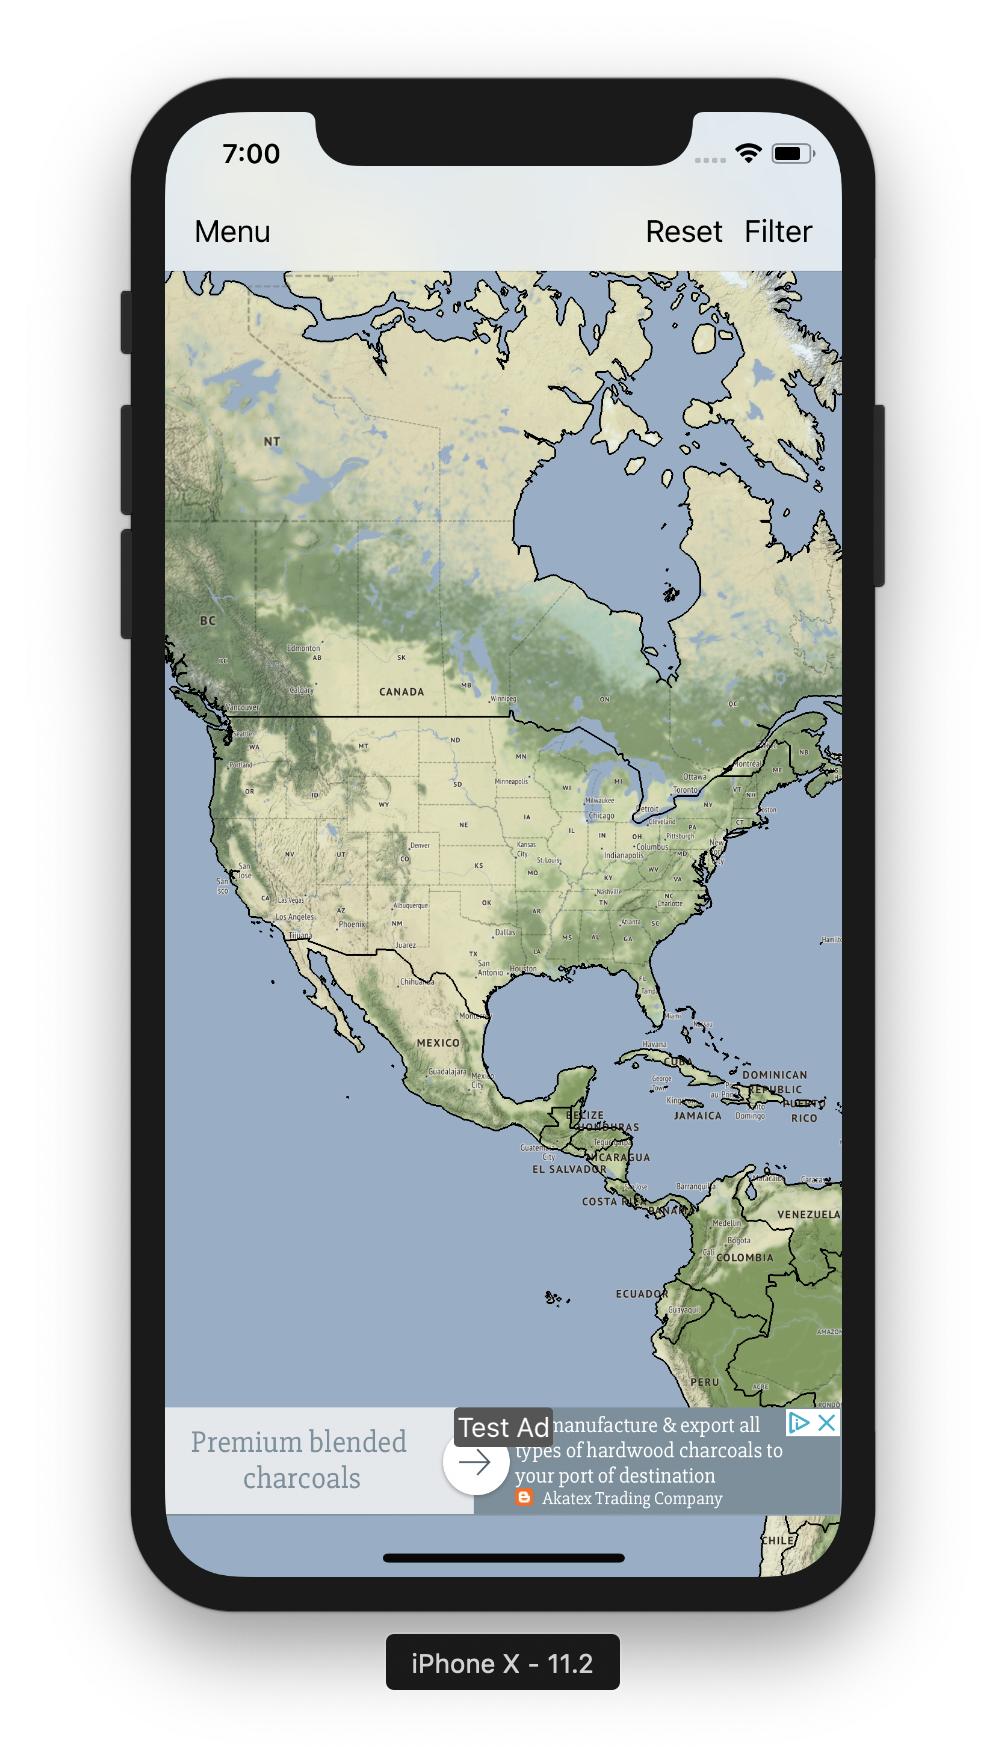
\includegraphics[width=0.5\linewidth]{figures/ch4/home.png}
            \caption{2D Map view}\label{fig:home_map}
        \end{minipage}
    \end{figure}
    
    The purpose of including Google Ads is to make money while giving the application to users for free. It also includes Google Ads at the bottom of the screen. Google AdMob for \gls{iOS} framework has been integrated to achieve this goal. Google has a lot of different types of ads and the one implemented is the banner view.

\subsubsection{Sliding Menu}

Sliding menu has been used in the app to make navigation easier for the user. It enables user to visit some of the key screens without any hustle. Figure~\ref{fig:side_menu_ch4} shows the sliding menu and the options it includes.

    \begin{figure}[H]
            \centering
            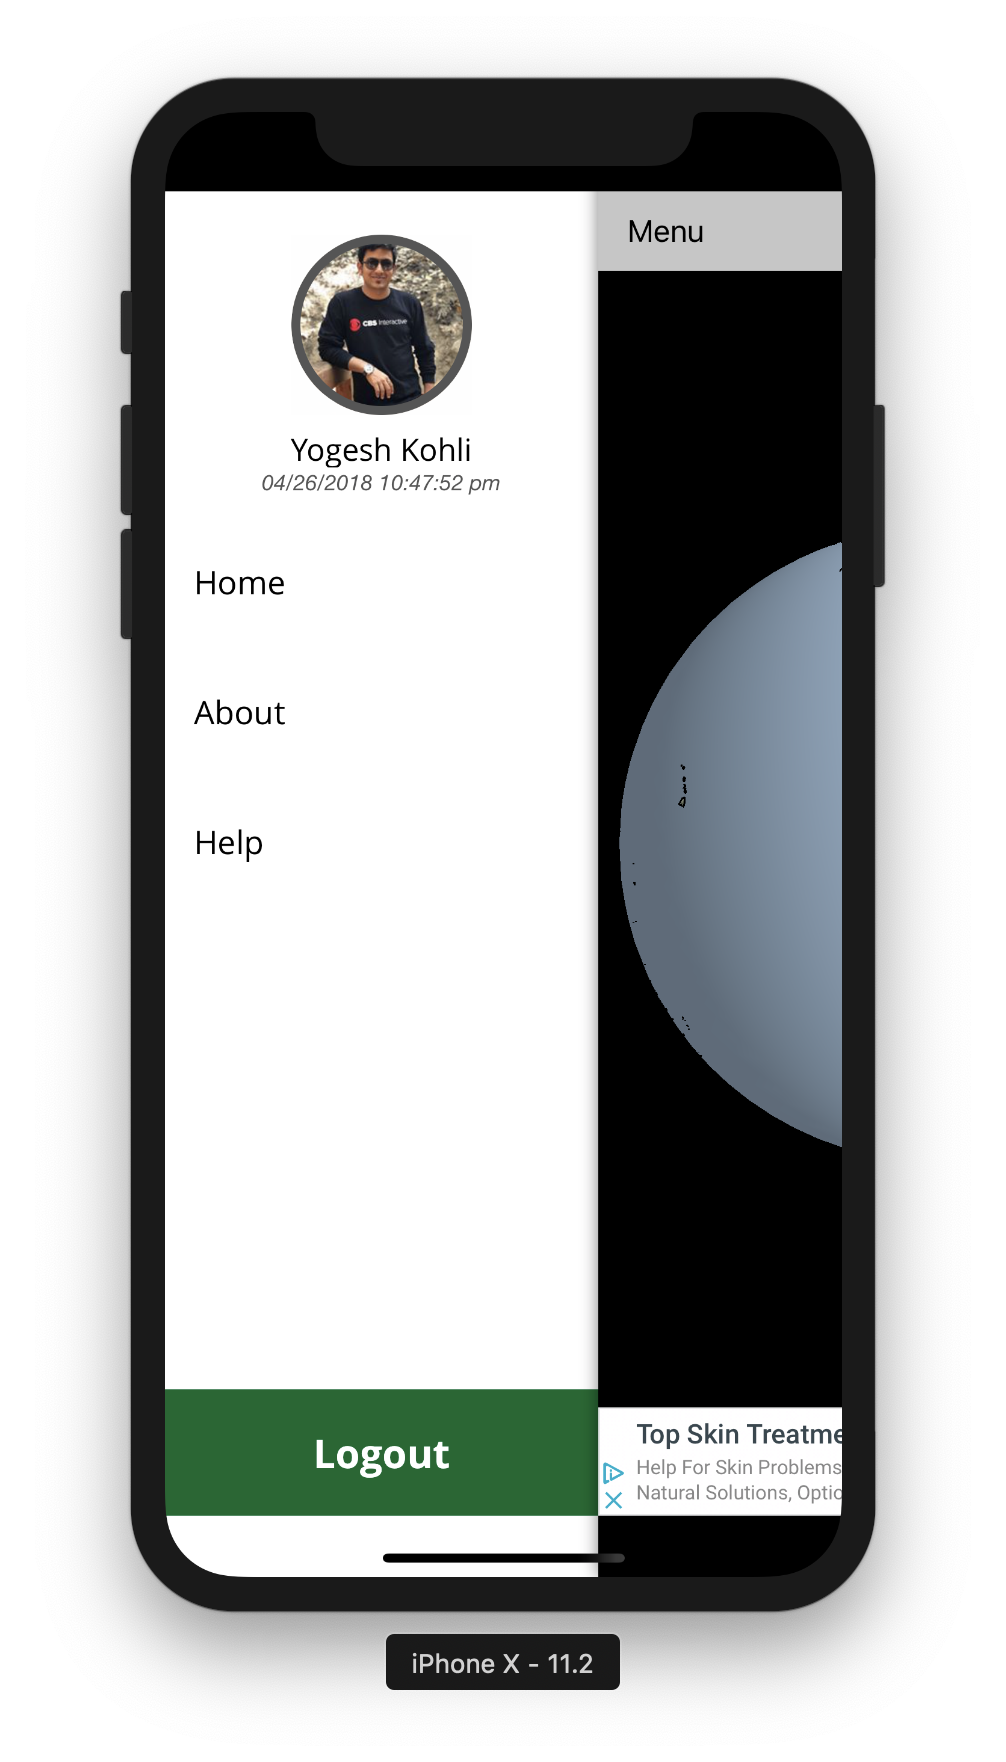
\includegraphics[width=0.25\linewidth]{figures/ch4/side_menu.png}
            \caption{\label{fig:side_menu_ch4} Sliding menu screen}
    \end{figure}

    User can easily navigate to the below mentioned screens.

    \begin{itemize}
    \item Home \\
    By tapping on home, it takes user to the home i.e landing page.
    
        \item About \\
            The main role of an about us page is to inform user about the organization and its tasks. This is a clear objective that all organizations need to satisfy in some form or another.
    
         \item Help \\
            The main reason for keeping help screen in slide menu is to provide user easier access to help in case of any query. He can follow certain steps and contact the developer / organization in case of any difficulties.
            
    \end{itemize}

\subsubsection{Filter process}

This is one of the most crucial part of the application which enables user to filter the data according to their needs. Filtering is being done on various parameters which are mentioned below. Filter screen is shown below in Figure~\ref{fig:filter_datatype}.

    \begin{figure}[H]
            \centering
            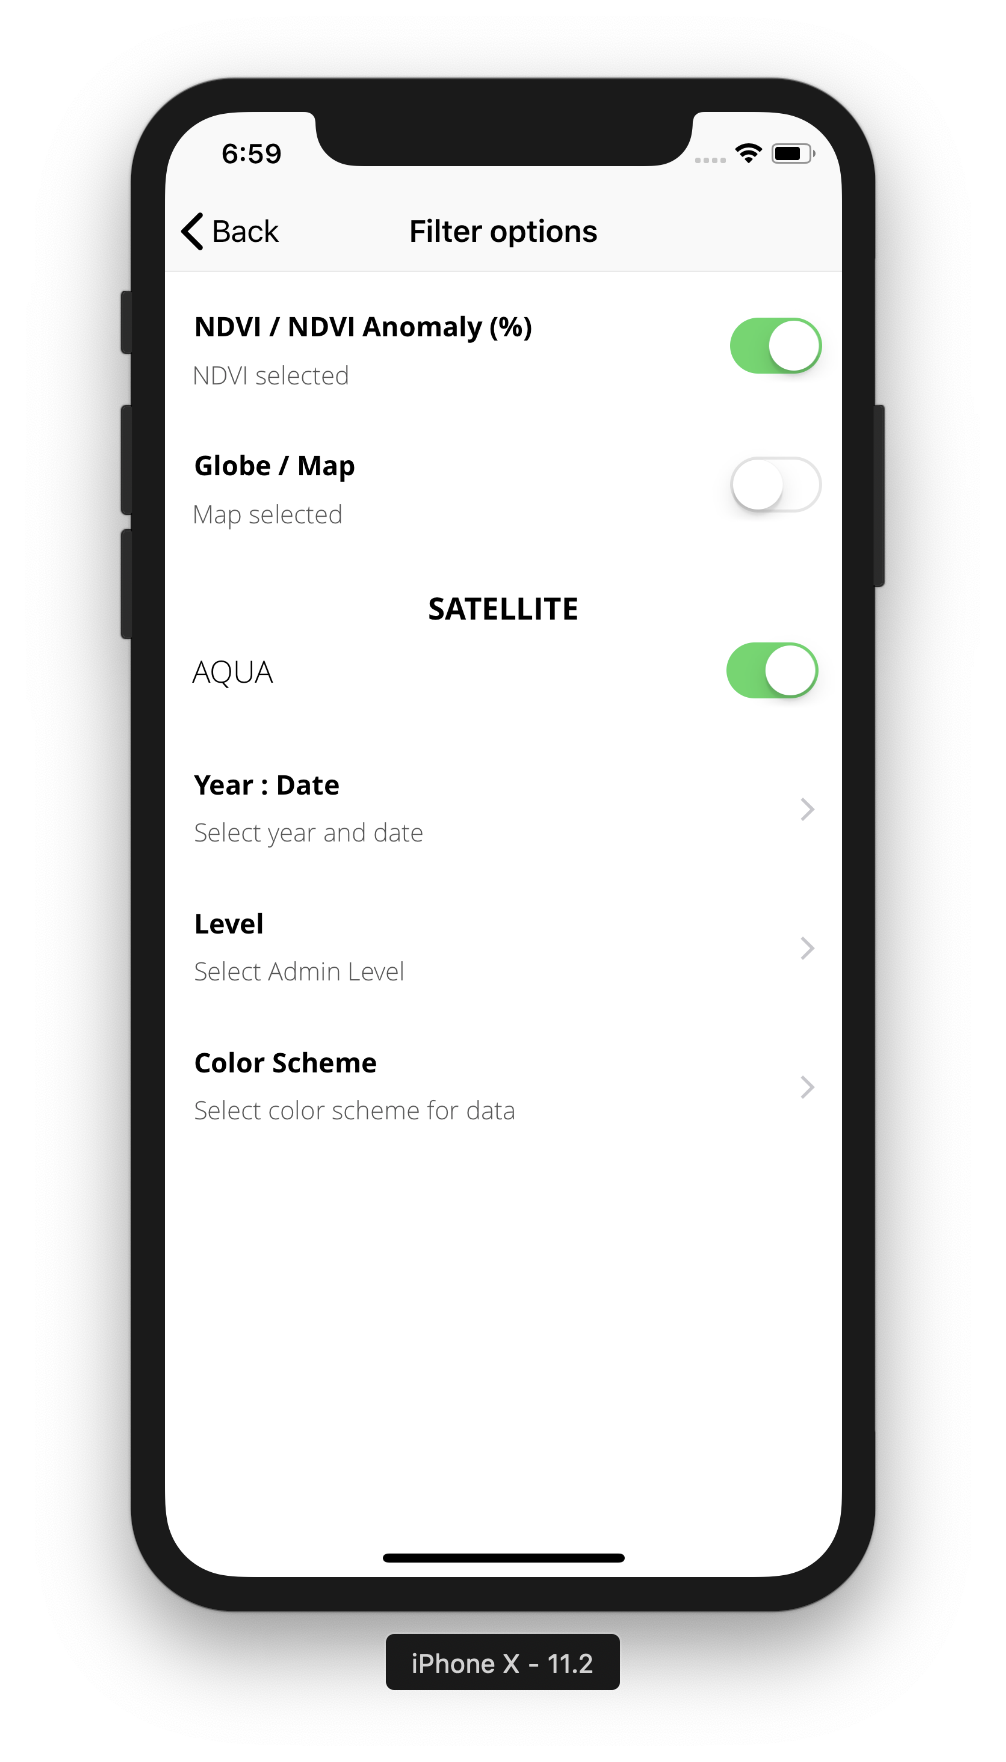
\includegraphics[width=0.25\linewidth]{figures/ch4/filter.png}
            \caption{\label{fig:filter_datatype} Filter screen showing different filtering options}
    \end{figure}

%FIGURE MANAGE PROPERLY - CORRECT IMAGES AFTER EDITING - BLURR HERE

\begin{itemize}
    \item \gls{ndvi} or Anomaly data \\
    This feature has been developed to give the user freedom of choosing the type of data he wants to visualize. A visual toggle - UISwitch has been used for this purpose to enable \gls{ndvi} or anomaly data. By default, \gls{ndvi} is selected. When the user changes the toggle to make it clear, the text under the heading also changes displaying what is being currently selected. 
  
    \item Globe or Map - Visualization medium \\
    User has the option to choose between 2D map view or Globe view.
    This has shown in Figure~\ref{fig:home_globe_mode} and Figure~\ref{fig:home_map}.

    \item Year and date \\
    Year and date list is to pick a specific date for which the user wants to see the data. Dates are only available after selecting the year from year list screen. The one thing to note here is that the year list and dates for that year is coming from server, so user will not see those dates or years which the data is not available.
    This dynamic thing has been done to increase user interaction and to give the stability to the app by making it dynamic as well as keeping in mind for future updates. Figure~\ref{fig:year_list_ch4} and Figure~\ref{fig:date_list_ch4} represents year and date list screens respectively.
    
    \newpage
    
    \begin{figure}[!htb]
        \begin{minipage}{0.5\textwidth}
            \centering
            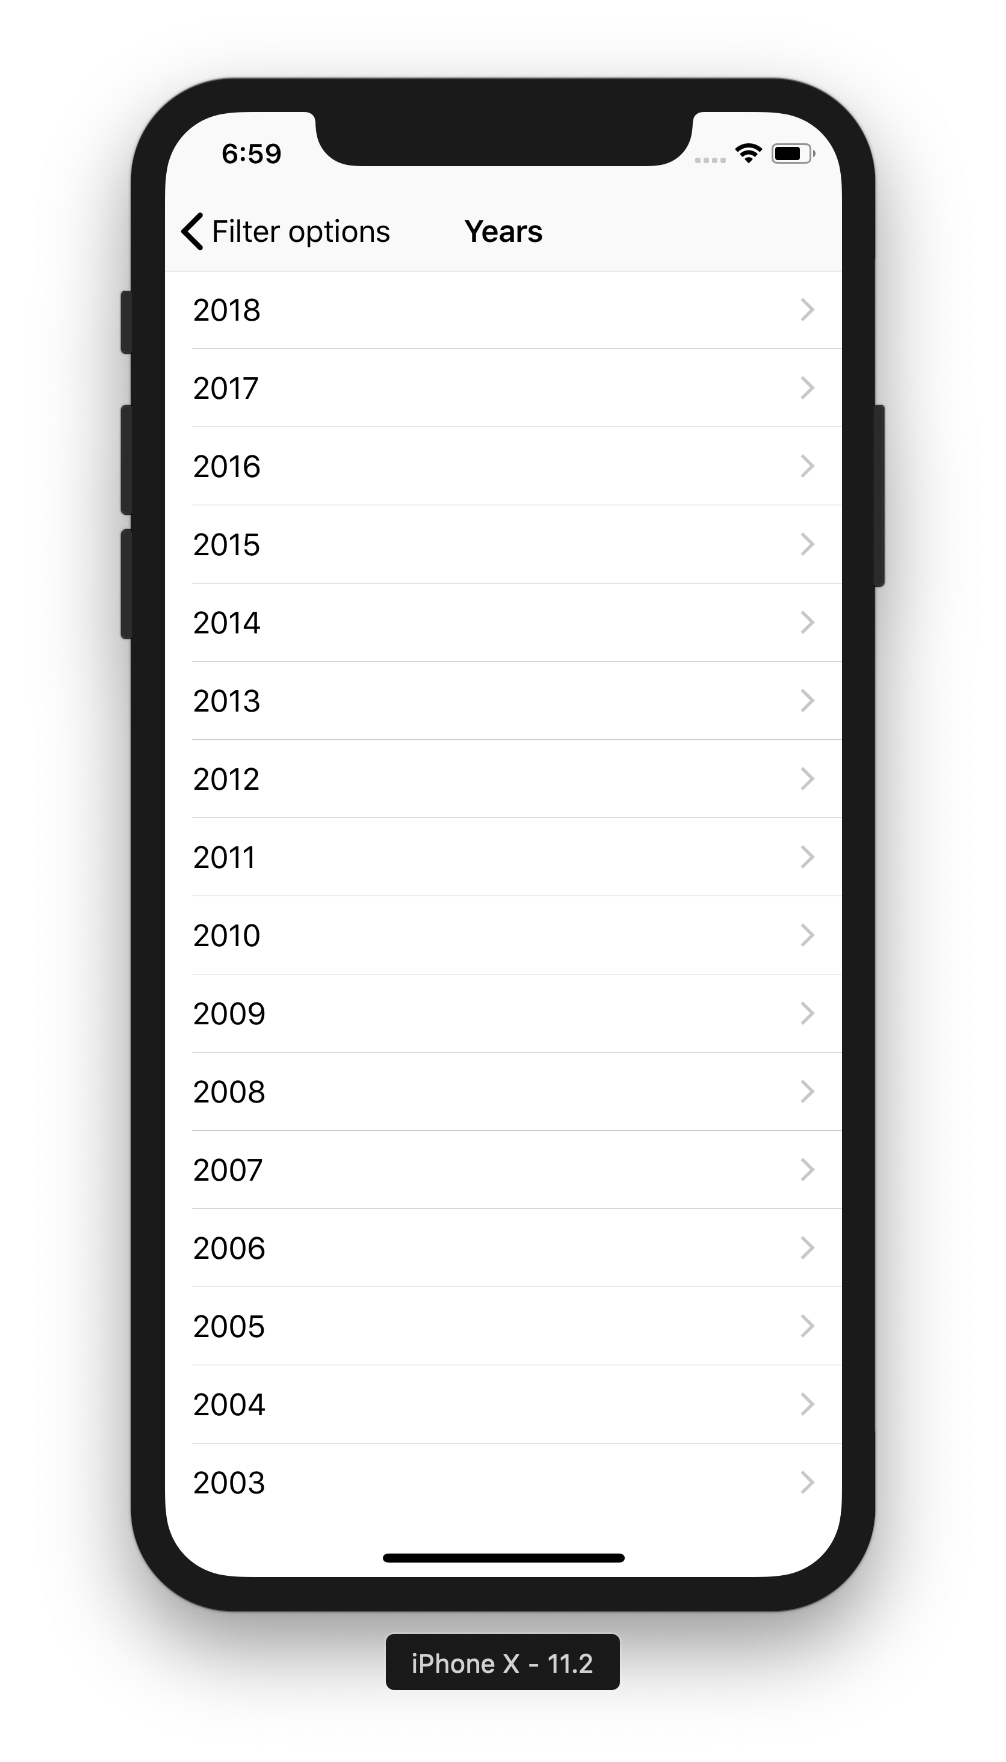
\includegraphics[width=0.5\linewidth]{figures/ch4/year_list.png}
            \caption{Year list}\label{fig:year_list_ch4}
        \end{minipage}\hfill
        \begin{minipage}{0.5\textwidth}
            \centering
            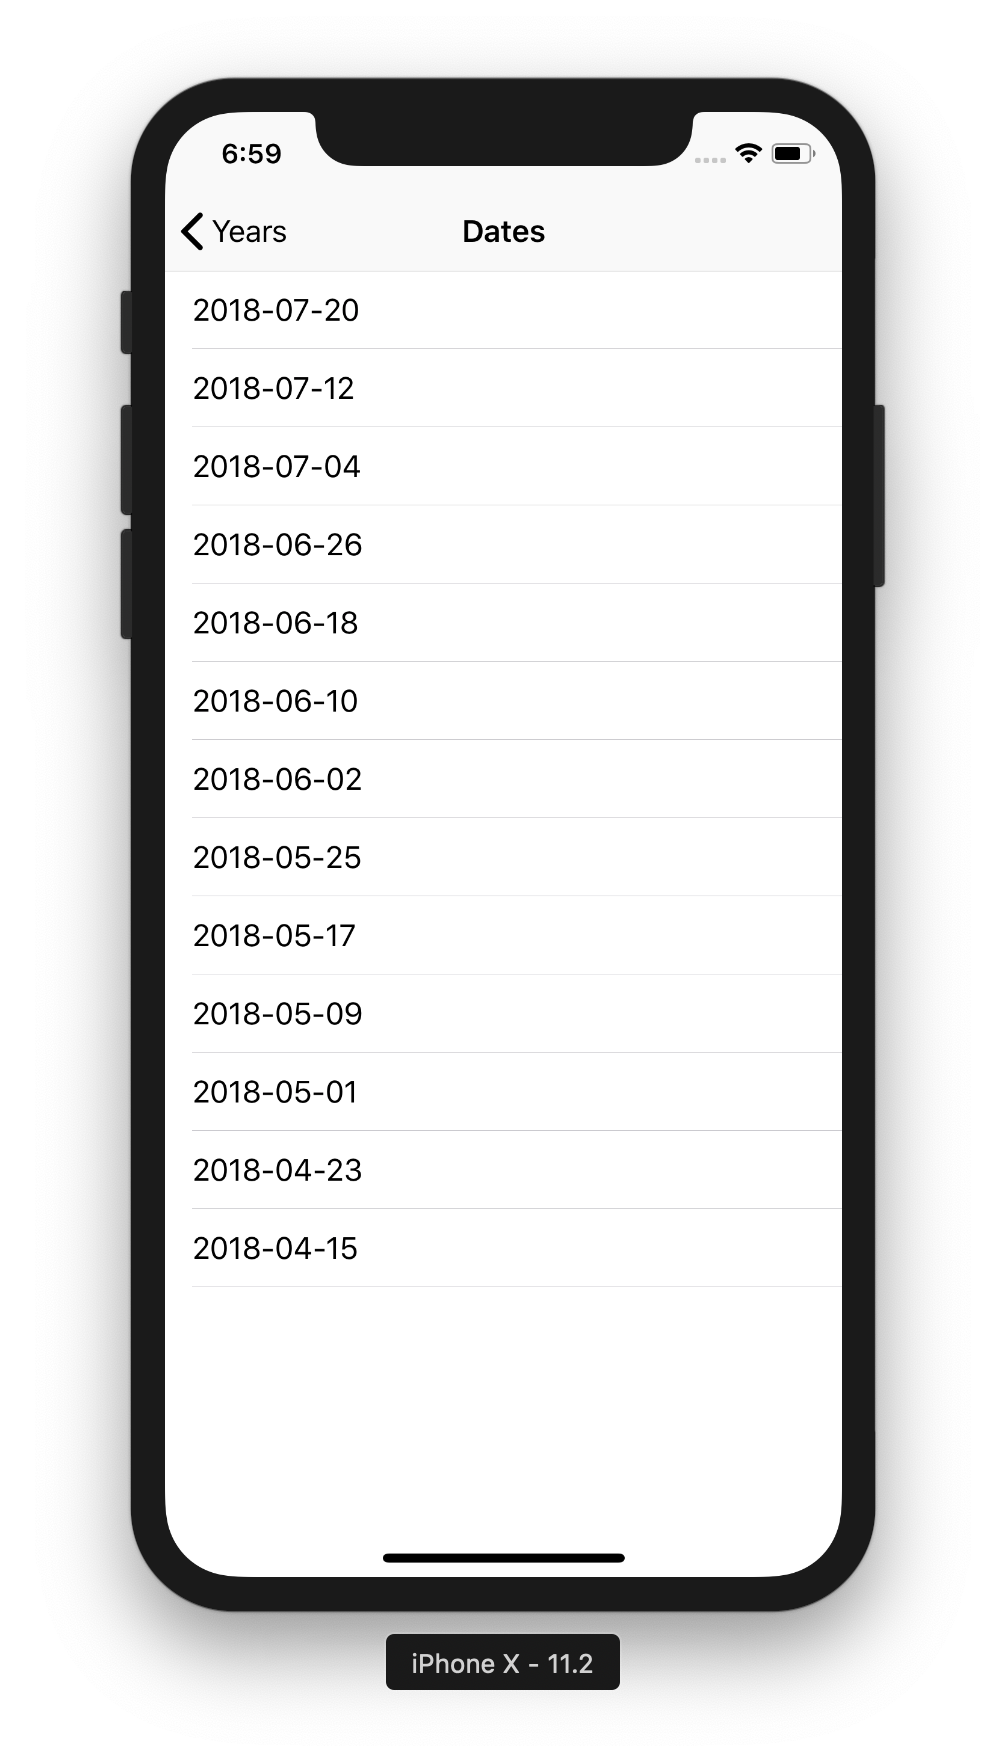
\includegraphics[width=0.5\linewidth]{figures/ch4/dates_list.png}
            \caption{Dates list after selecting year}\label{fig:date_list_ch4}
        \end{minipage}
    \end{figure}
   
    \item Color scheme
    
    %add images of color schemes used in this project too
    
    This is an additional feature which has given to the application to make it visually rich. It enables users to view data with different color palette schemes. Remember, the color palettes are custom made and stored locally in \gls{json} files according to the \gls{ndvi} range. Figure~\ref{fig:color_scheme_screen} shows color palette options available in the app. Users just have to select any of the available options and tap apply to make the commit of their choice.
    
     \begin{figure}[H]
            \centering
            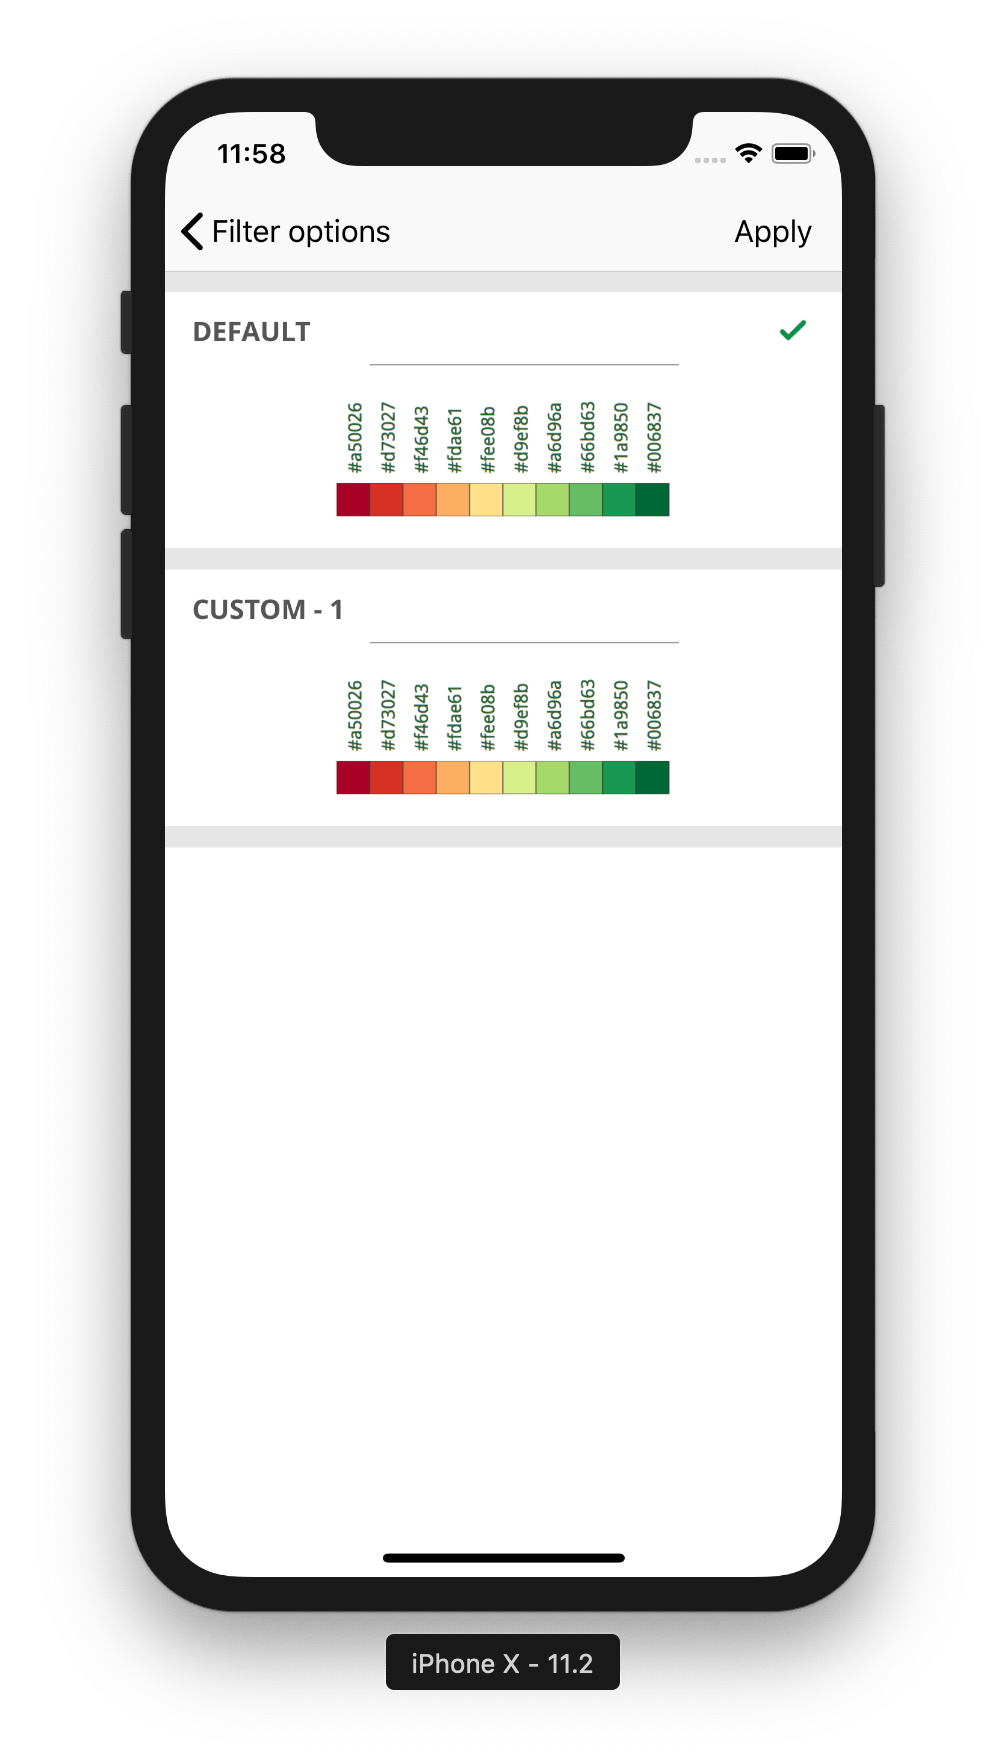
\includegraphics[width=0.25\linewidth]{figures/ch4/color_scheme.png}
            \caption{\label{fig:color_scheme_screen} Color scheme screen}
    \end{figure}
        
    Figure 4.23 shows an example of part of one entrie of \gls{json} file.
    
    \begin{figure}[H]
            \centering
            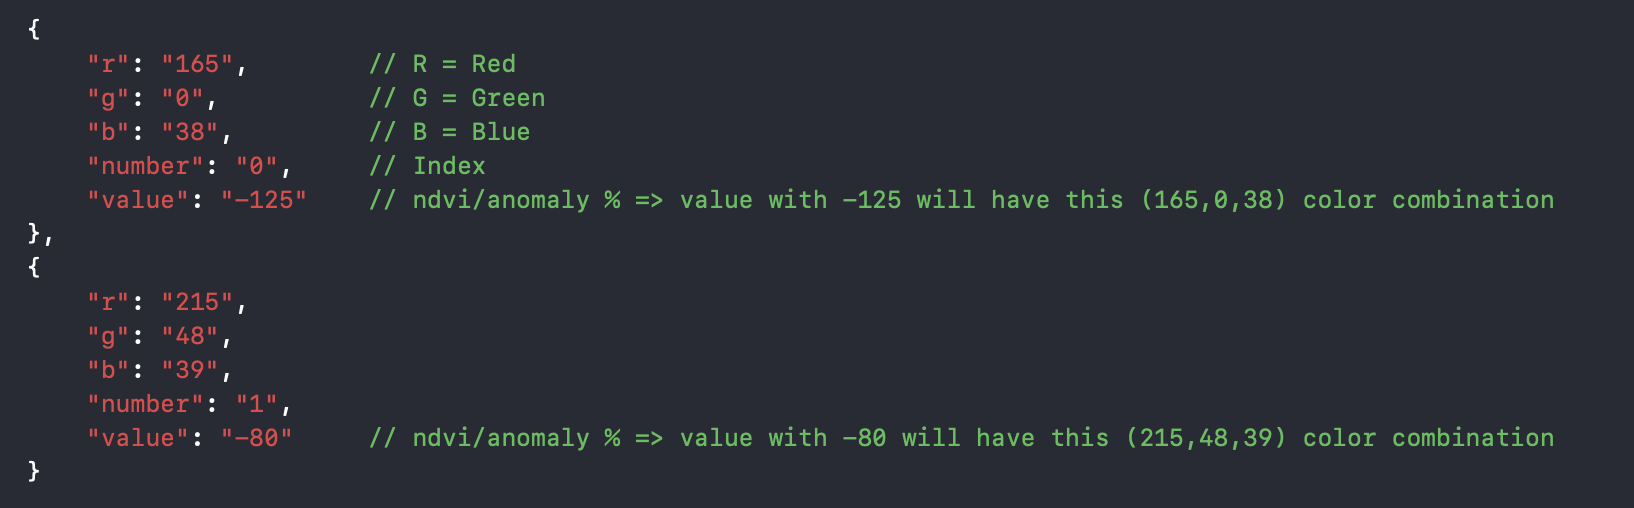
\includegraphics[width=1.0\linewidth]{figures/ch4/color_map_final.png}
            \caption{\label{fig:color_json} Sample JSON of custom created colormap file}
    \end{figure}

\end{itemize}


\section{Back-end of the app}

\subsection{Process of getting data from NASA's server}

A significant advance procedure of getting information from NASA's server and inserting information into the PostgreSQL, was developed and implemented using the python 3.6. The data on Nasa's server is in \gls{geoTiff} format. It is important to note that \gls{geoTiff} files stored in their server are compressed via zip.

According to Wikipedia, \gls{geoTiff} is a public domain metadata standard which allows georeferencing information to be embedded within a TIFF file. The potential additional information includes map projection, coordinate systems, ellipsoids, datums, and everything else necessary to establish the exact spatial reference for the file \cite{GeoTIFF_Wikipedia}. Figure~\ref{fig:geotiff} represents NASA's data bundled in \gls{geoTiff} file.

    \begin{figure}[H]
            \centering
            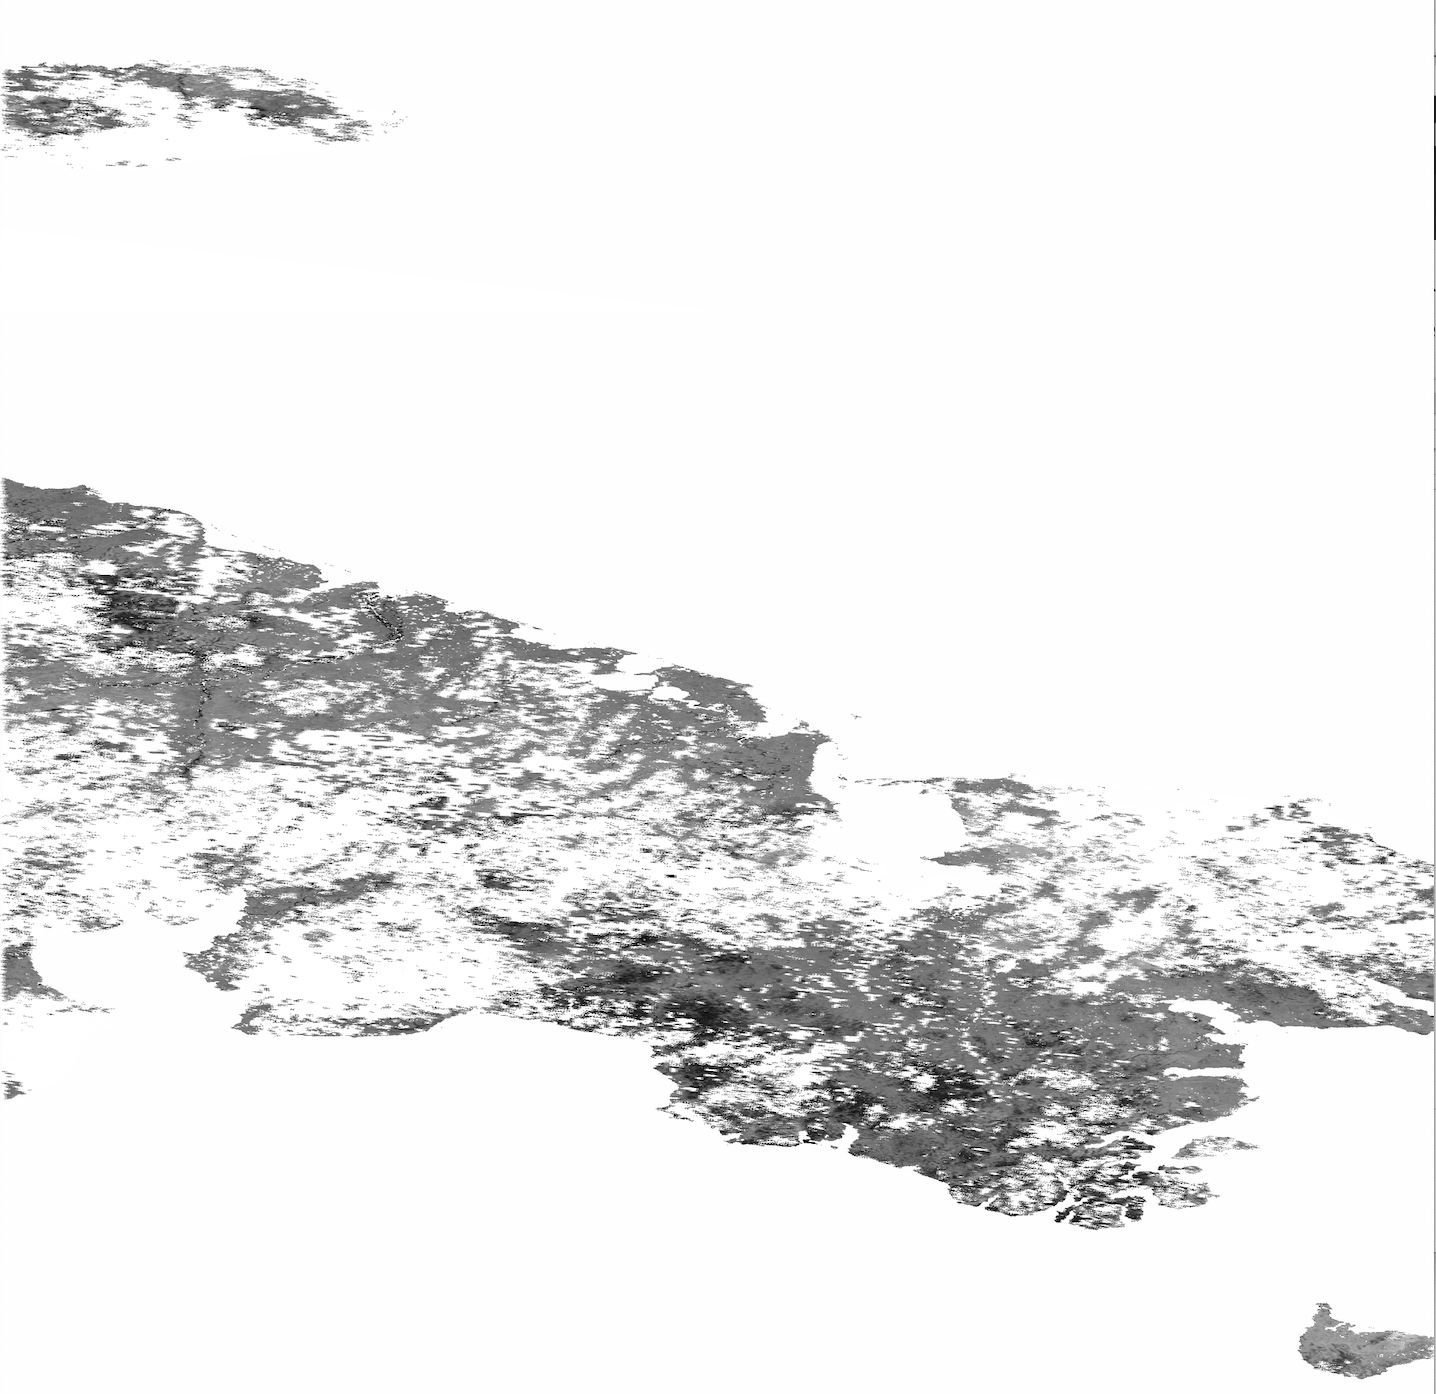
\includegraphics[width=0.35\linewidth]{figures/ch4/geotiff.png}
            \caption{\label{fig:geotiff} Sample of NASA's NDVI GeoTiff data file}
    \end{figure}

    Steps taken to get the raw data from this \gls{geoTiff} file, process the data and finally to store that data to a database are as follows:
    
    \begin{itemize}
        \item Find the beginning of the 8-day set and make your string formatted according to Nasa's file name format.
        
        \item Open zip without decompressing. If unzipped, the record gets 16 times bigger in size which at last puts weight on processor to process the file.
        
        \item Read the file row by row one at a time and process the data accordingly by converting data points to \gls{ndvi} values.
        
        \item Customizing the data according to the database structure and finally storing that data.
    \end{itemize}

\subsection{Web services required for JSON parsing between database and the front-end}

\textbf{RESTful web services} are built to work best on the Web. Representational State Transfer (REST) is an architectural style that specifies constraints, such as the uniform interface, that if applied to a web service induce desirable properties, such as performance, scalability, and modifiability, that enable services to work best on the Web. In the REST architectural style, data and functionality are considered resources and are accessed using Uniform Resource Identifiers (URIs), typically links on the Web. The resources are acted upon by using a set of simple, well-defined operations. The REST architectural style constrains an architecture to a client/server architecture and is designed to use a stateless communication protocol, typically HTTP. In the REST architecture style, clients and servers exchange representations of resources by using a standardized interface and protocol. \cite{RESTful_web_services} \\

\textbf{\gls{json}} is a lightweight information parser. It is a content arrangement that is totally dialect free yet utilizes traditions that are recognizable to software engineers of the C-group of dialects, including C, C++, Java, JavaScript, PHP, Python, and numerous others. These properties make JSON a better information exchange dialect and helps developers to transfer data between the server and the front-end of any software. The language used for creating web services is \textbf{\gls{php}}. List of web services creates for the project are mentioned below.

\begin{itemize}
    \item \textbf{dbcon.php} \\
    It contains a database connection function for connecting to PostgreSQL database. \textbf{pg\_connect} function has been used to connect to the database. It opens up a connection to the database specified by the credentials of the server in the connection string. \\
    
    \item \textbf{credentials.php} \\
    It contains all the services related to login, register and forgot password. \\
    
    \item \textbf{getdata.php} \\
    It has all the services for the ndvi data including filtering process. \\
\end{itemize}

\section{Using the app}

\subsection{Data Visualization}

Process of displaying the data is described as below.

\begin{itemize}
    \item Select any filter options if desired.
    \item Select year and date.
    \item Tap on any country or region to see the data at the selected locations.
\end{itemize}
This section contains all three cases of Admin Level and their effect on Home screen that is data visualization. Different types of level data are mentioned below.

\begin{itemize}
    \item \textbf{Admin Level 0 - Country Wise} \\
    Each country has been colored with the mean NDVI value for a particular date, calculated using the appropriate formula.
    
     \begin{figure}[!htb]
        \begin{minipage}{0.45\textwidth}
            \centering
            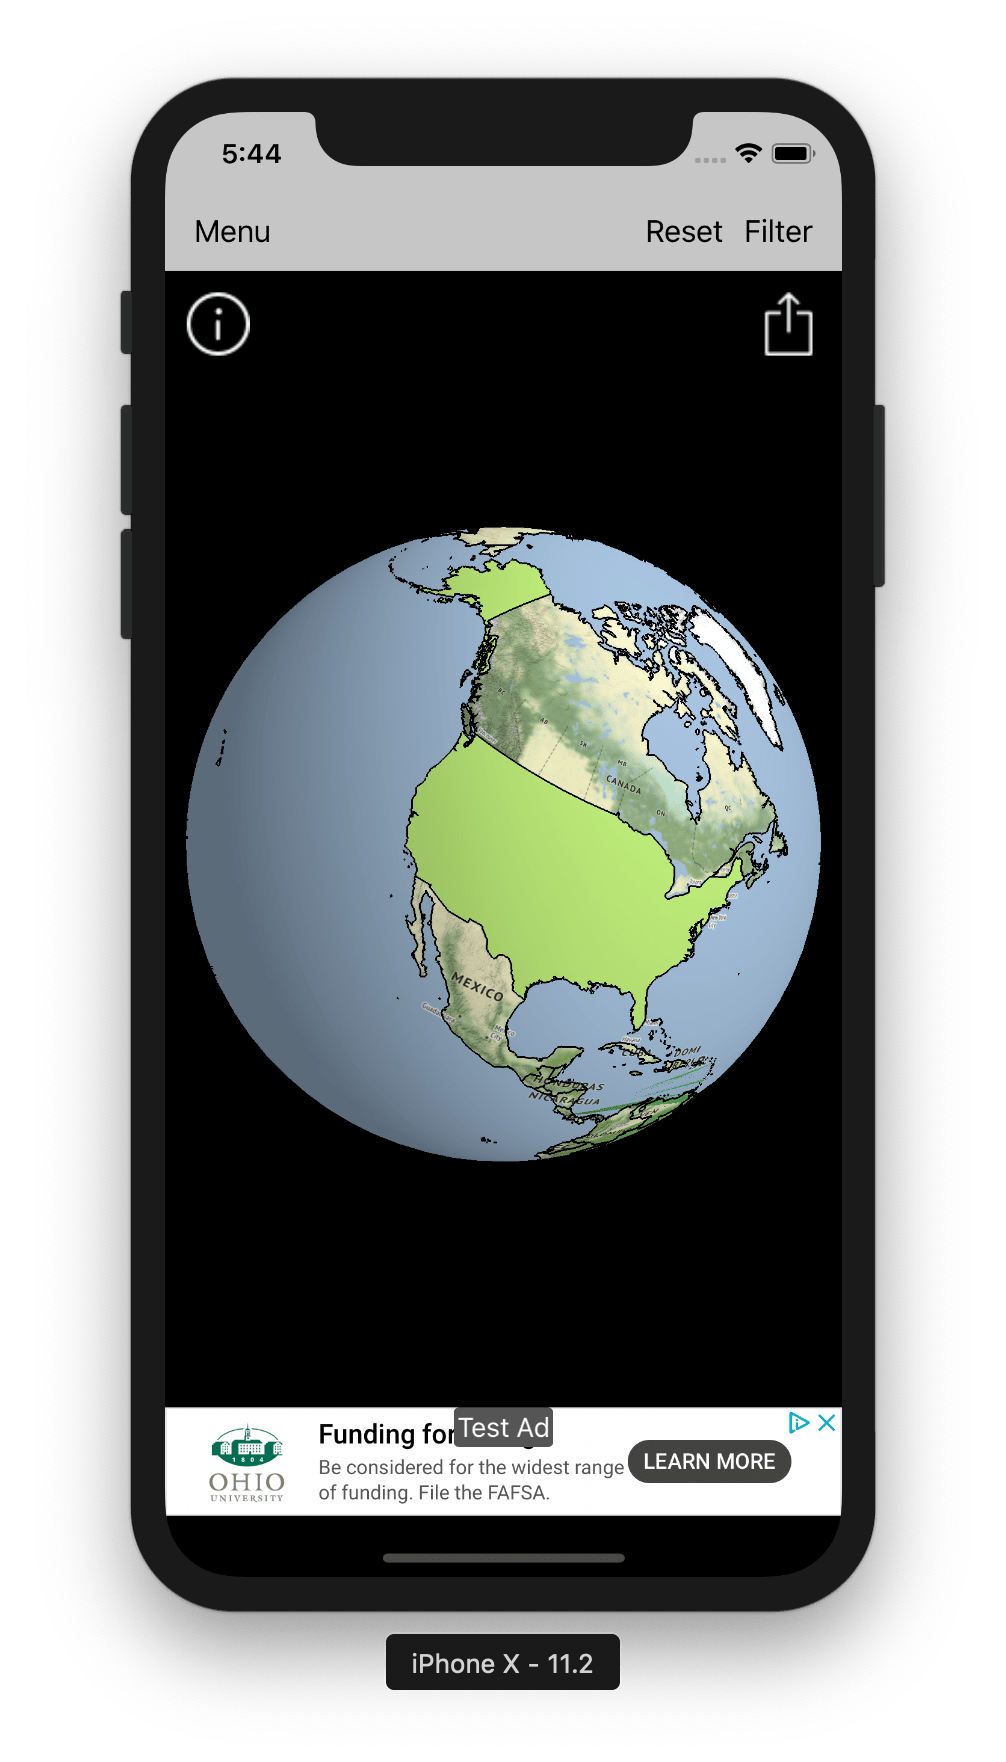
\includegraphics[width=0.5\linewidth]{figures/ch4/admin_level_0_a.png}
            \caption{Admin level 0 mean NDVI shown country wise - United States}\label{Fig:admin_level_0_a}
        \end{minipage}\hfill
        \begin{minipage}{0.5\textwidth}
            \centering
            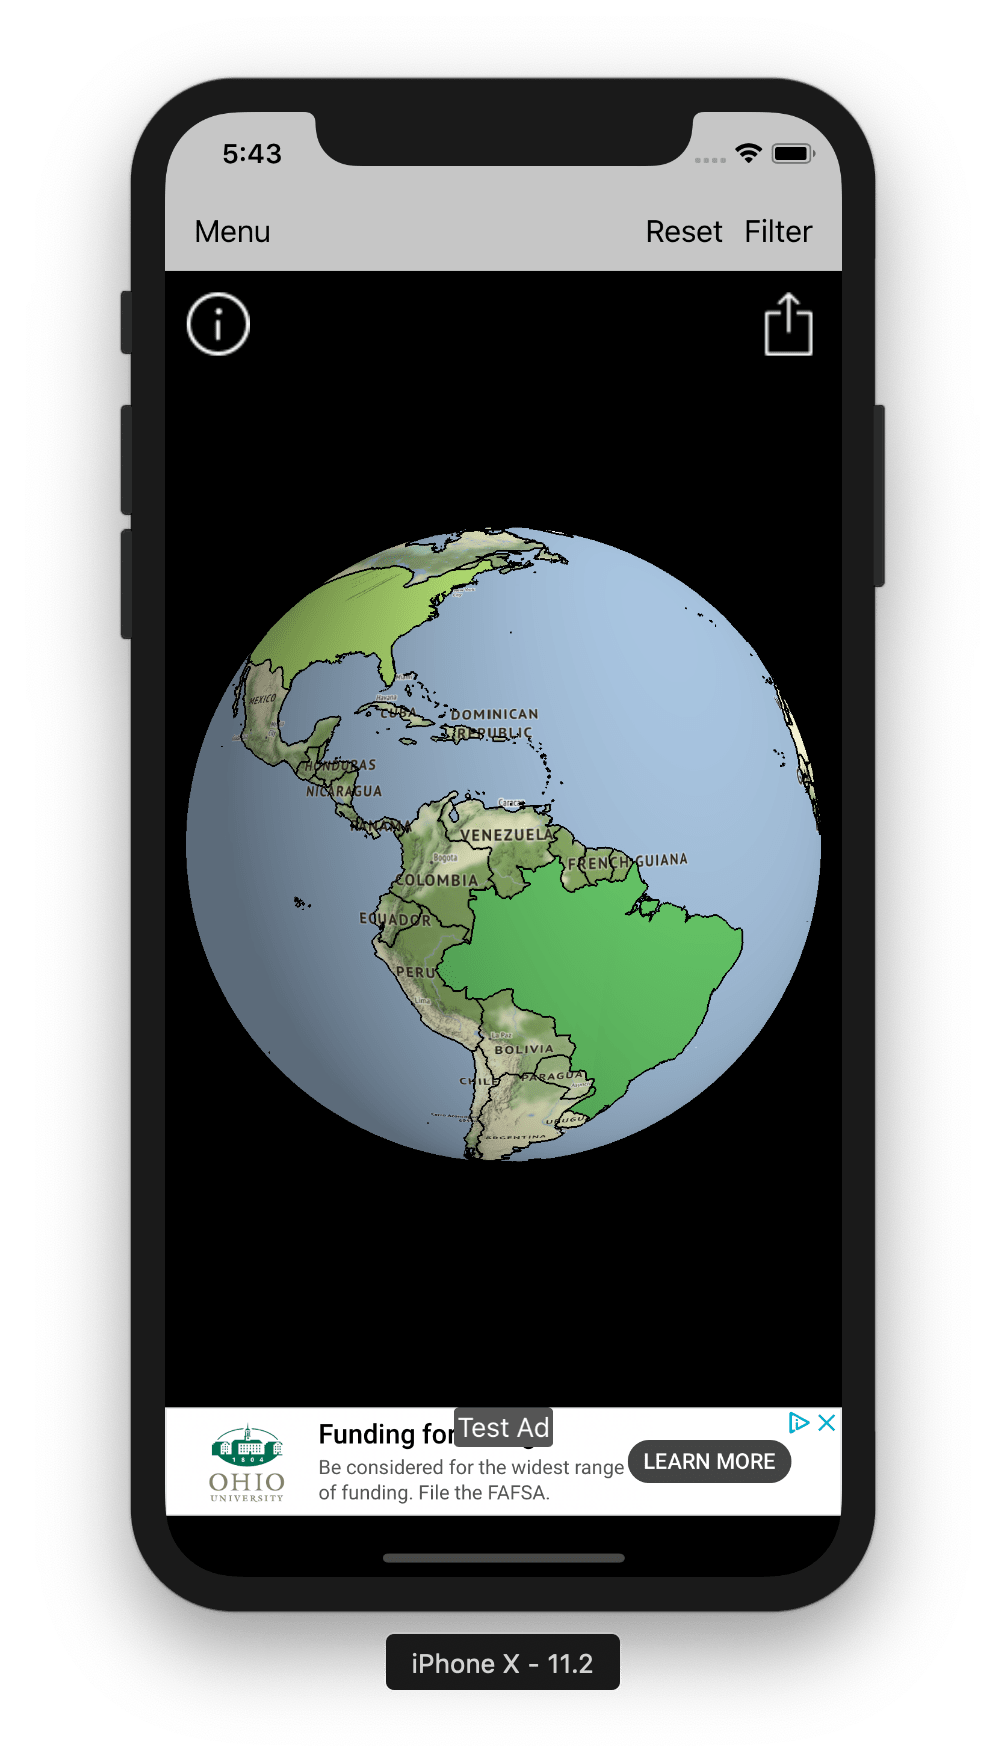
\includegraphics[width=0.45\linewidth]{figures/ch4/admin_level_0_b.png}
            \caption{Another example of Admin level 0 mean NDVI shown country wise}\label{Fig:admin_level_0_b}
        \end{minipage}
    \end{figure}
    
    \item \textbf{Admin Level 1 - State Wise} \\
    Each state of a country has been colored with the mean value of \gls{ndvi} for the specified date, as shown in the figure below.
    
    \begin{figure}[!htb]
        \begin{minipage}{0.45\textwidth}
            \centering
            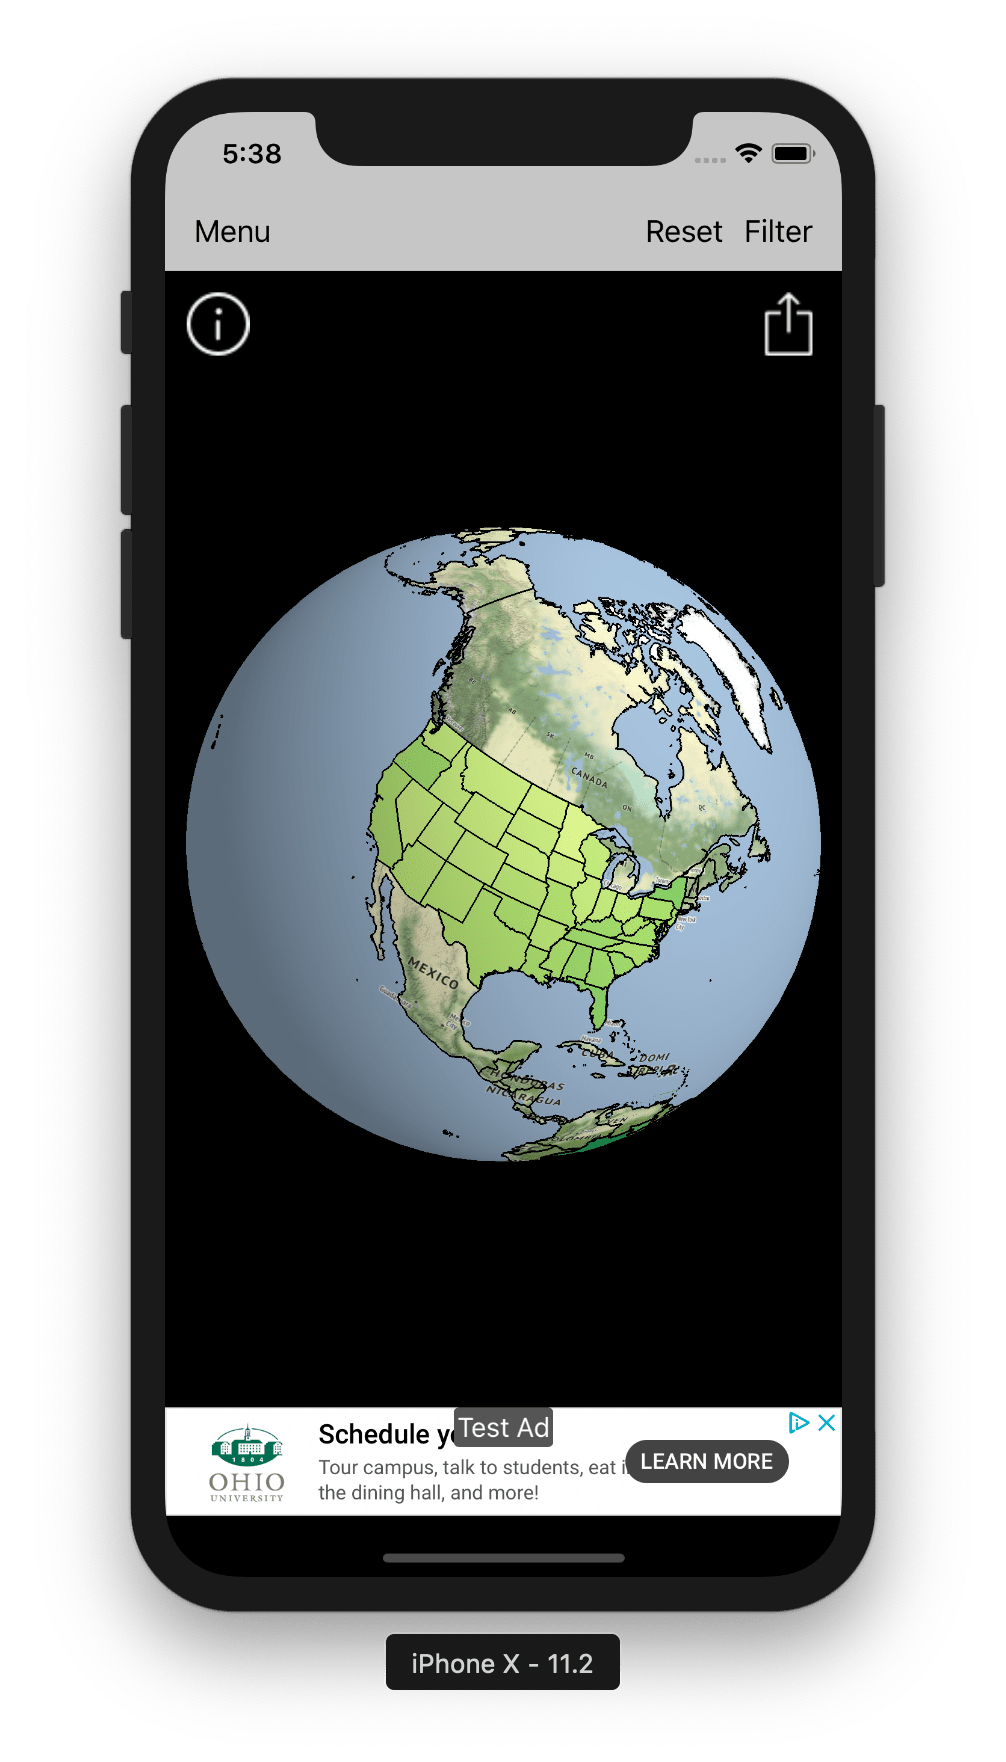
\includegraphics[width=0.5\linewidth]{figures/ch4/admin_level_1_a.png}
            \caption{Admin level 1 mean NDVI shown state wise - United States}\label{Fig:admin_level_1_a}
        \end{minipage}\hfill
        \begin{minipage}{0.5\textwidth}
            \centering
            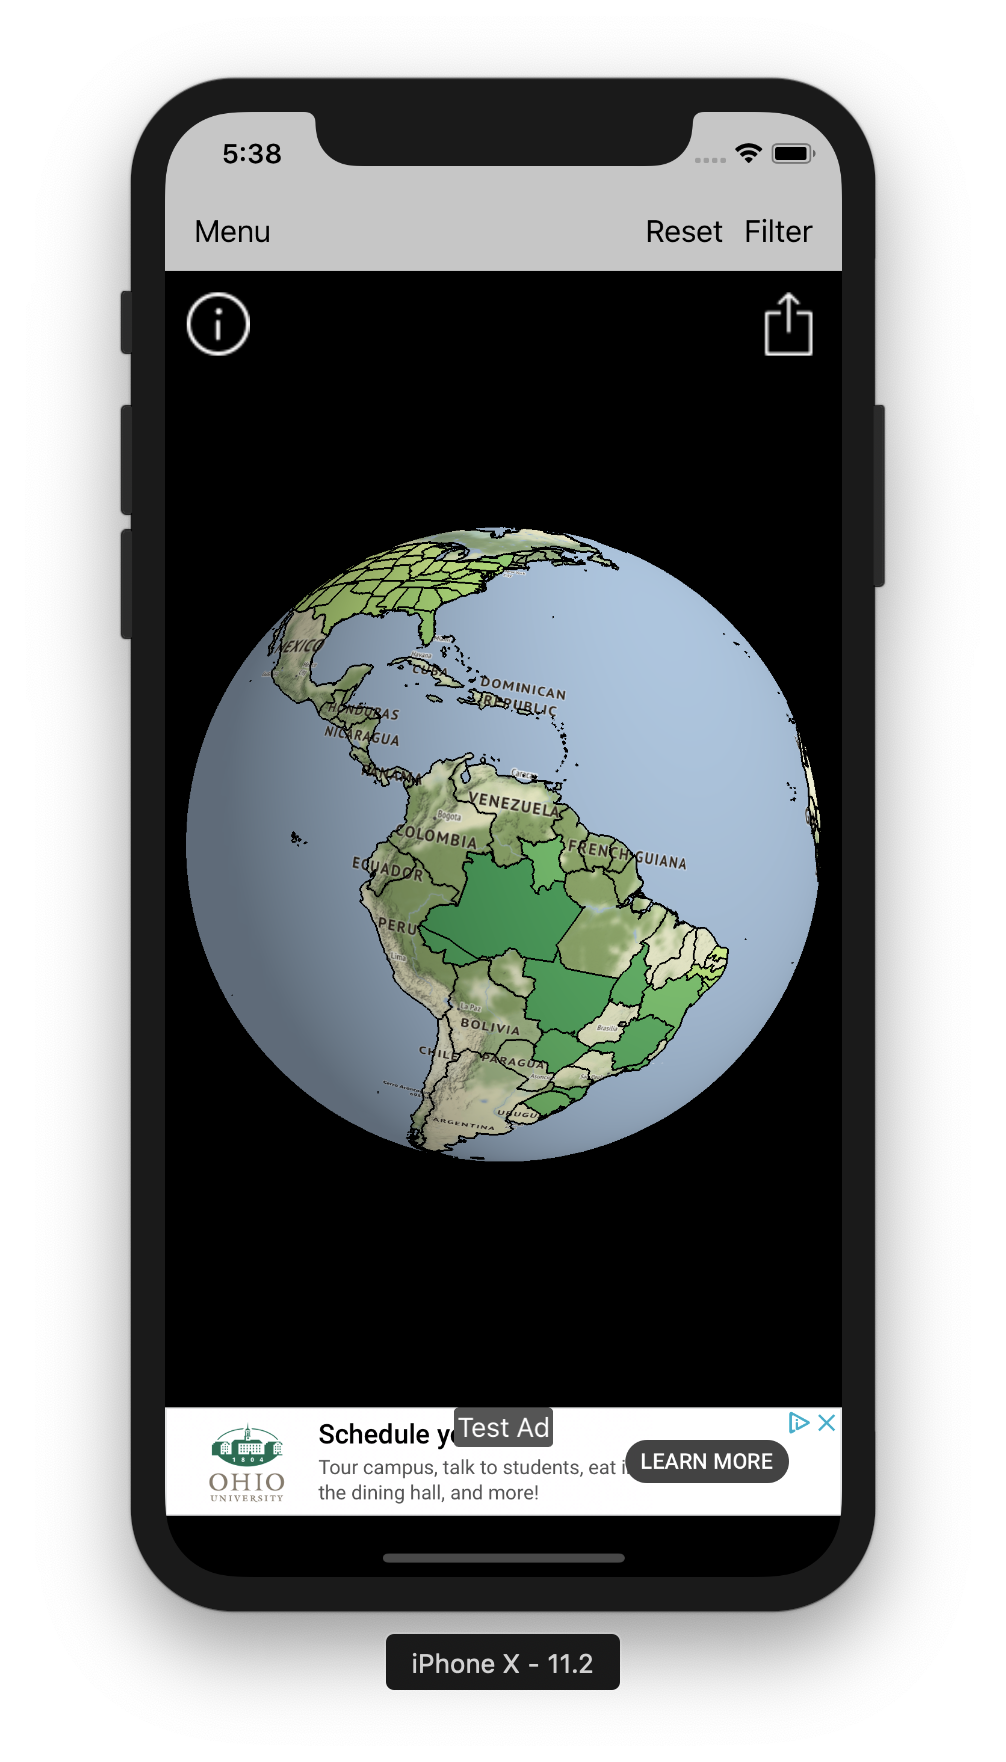
\includegraphics[width=0.45\linewidth]{figures/ch4/admin_level_1_b.png}
            \caption{Another example of Admin level 1 mean NDVI shown state wise - Brazil}\label{Fig:admin_level_1_b}
        \end{minipage}
    \end{figure}
  
    \item \textbf{Admin Level 2 - District Wise} \\
    District mean values has been calculated and district regions have been colored accordingly.
    
     \begin{figure}[H]
            \centering
            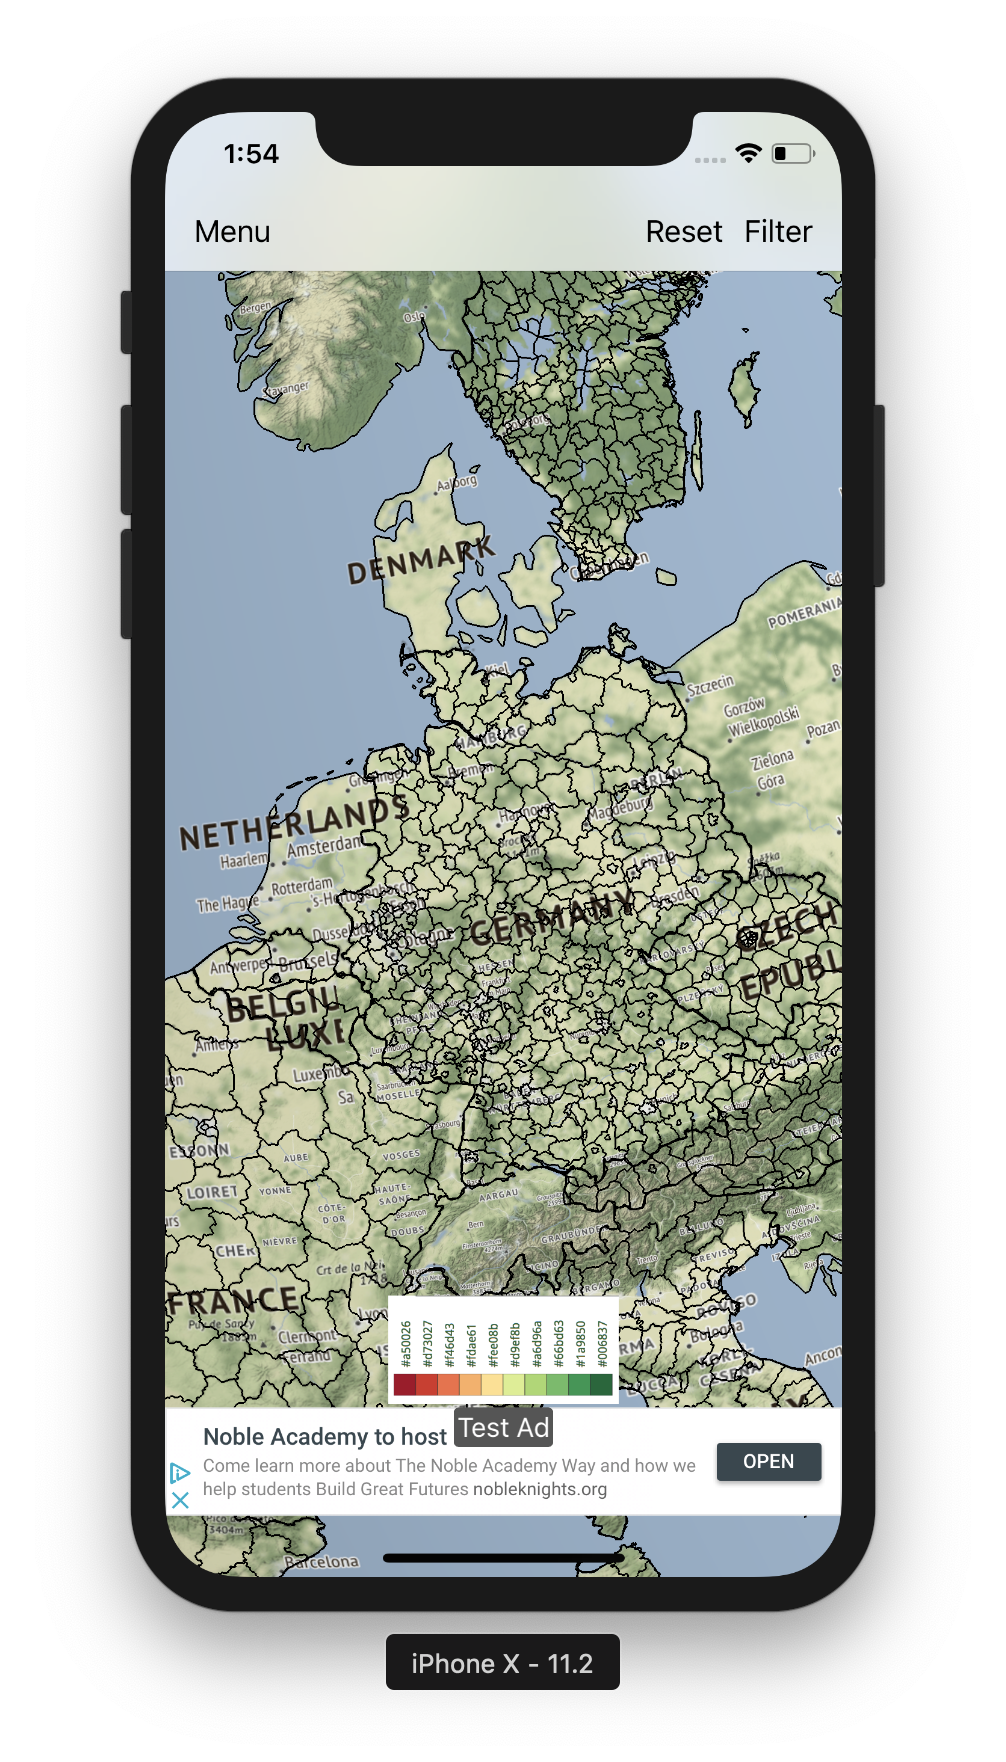
\includegraphics[width=0.25\linewidth]{figures/ch4/admin_level_2.png}
            \caption{\label{fig:admin_level_2_visual}  Admin level 2 data visualization}
        \end{figure}
    
\end{itemize}


\section{APIs, Softwares, Design pattern and Languages Usage}

\subsection{APIs Usage}

Major APIs used in the project to make the application better are explained below.

\begin{itemize}
    \item \textbf{Alamofire} - HTTP Networking Library
    
    Alamofire is a Swift-based HTTP networking library for \gls{iOS} and \gls{macOS}. It gives a rich interface over Apple's Foundation organizing stack that disentangles various basic networking assignments\cite{Alamofire}. It can be found here \url{https://github.com/Alamofire/Alamofire} \\
   
    \item \textbf{WhirlyGlobe} - Globe SDK
    
    Focusing on mobile technology based on OpenGL ES. It is an open source library which is utilized in a wide assortment of guide applications. The \gls{sdk} 3D intelligent globe and a 2D map for \gls{iOS} \cite{WhirlyGlobe}. It is important to mention that this library has been customized according to the needs of the application. Classes has been modified by adding some delegate methods which enables developers to have more control on the visualization. It can be found here  \url{https://github.com/mousebird/WhirlyGlobe} \\
    
    \item \textbf{SwiftCSVExport} - Exporting data
    
    Swift CSV Export is lightweight and rich. It enables developers to create, read and compose CSV records easily\cite{Swift_CSV_Export}. This library has been utilized to change over the \gls{json} dictionary to the required objects which it takes and to package the information into CSV fil and send it through email. Remember, this library has also been customized and used according to the data type. It can be found here 
    - \url{https://github.com/vigneshuvi/SwiftCSVExport} \\ 
    
\end{itemize}

\subsection{Softwares used in the project}

List of Softwares used in the project with their significance are mentioned below.

\begin{itemize}
    \item \textbf{Xcode}
    It's an \gls{ide} by Apple, used for development of the app. \\
    
    \item \textbf{Axure RP 8}
    Used for creating wireframes. \\
    
    \item \textbf{Bracket}
    It's a text editor used to code web services in \gls{php}. \\
    
    \item \textbf{FileZilla}
    It's a cross platform \gls{ftp} application used to update and transfer files to server. \\
    
\end{itemize}


\subsection{Design Pattern used}

\textbf{\gls{mvc}} is a software design configuration used to create user interfaces, it is therefore a common choice for architecting web apps. In general, it separates out the application logic into three parts, helping modularity and simplicity of teamwork and reprocess. Likewise applications become more flexible and friendly to iterations \cite{MVC}. \\
According to Apple's documentation about design patterns, \gls{mvc} is a design pattern used for Cocoa applications. It provides reusability and extensibility to the applications. It is composed of three layers which are model, view and controller \cite{MVC_Apple}. It is shown in the Figure~\ref{fig:mvc}.

\begin{itemize}
    \item \textbf{Model} \\
    The Model is the place your data lives. Parsers and networking code typically live there. \\
    
    \item \textbf{View} \\
    The View layer is the essence the application. Its classes are commonly reusable, since there aren't any logical operation being performed on it. The UILabel presents message on the screen, besides being effectively reusable. \\
  
    \item \textbf{Controller} \\
    The Controller intercedes between the view and the model, normally through the delegation concept. In the perfect situation, the controller element won't know the solid view it's managing. Instead it will speak with an abstraction with the help of protocols. An exemplary model is the manner in which a UITableView interacts with its data source through the UITableViewDataSource protocol. \\
    
\end{itemize}

    \begin{figure}[H]
            \centering
            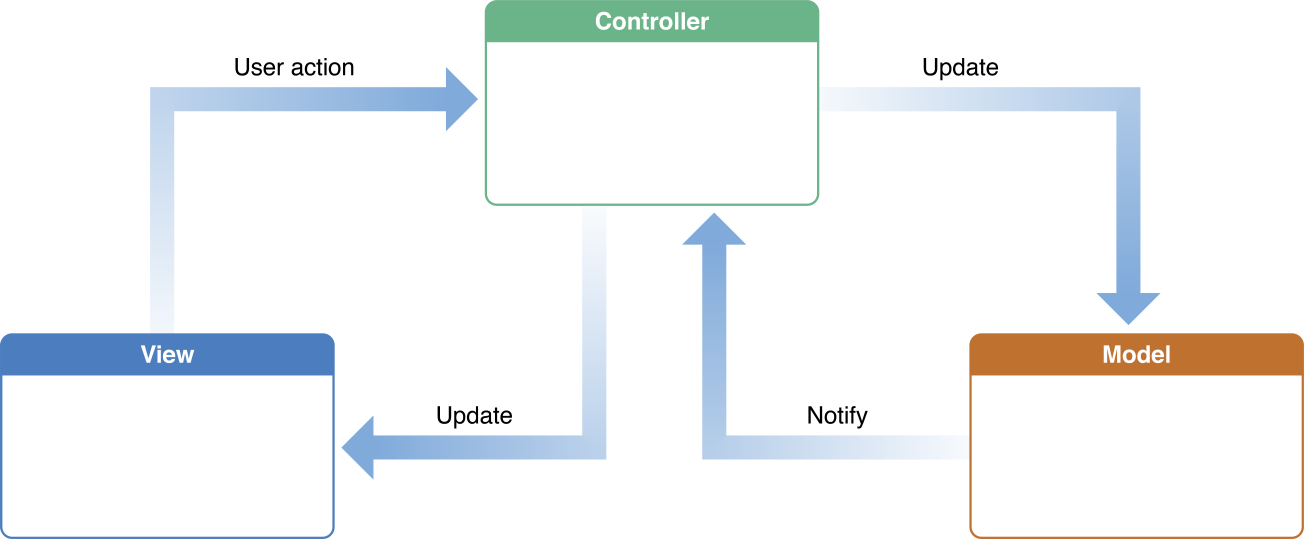
\includegraphics[width=1.0\linewidth]{figures/ch4/mvc.png}
            \caption{\label{fig:mvc} MVC Architecture \cite{MVC_Apple}}
        \end{figure}

\subsection{Software Languages used in the project}

List of software languages used in the process are mentioned below.

\begin{itemize}
    \item \textbf{Swift 4.1} - Used for development of iOS app \\
    \item \textbf{PHP} - Used for data parsing between server and the app \\
    \item \textbf{Python} - Used for getting data from \gls{nasa}'s server and storing it in database. \\
    \item \textbf{R} - Used for implementing \gls{svd} for analysis. \\
\end{itemize}
